\documentclass{scrartcl}
    % General document formatting
    \usepackage[margin=0.7in]{geometry}
    \usepackage[parfill]{parskip}
    \usepackage[utf8]{inputenc}
    \usepackage[english]{babel}
    
    % Related to math
    \usepackage{amsmath,amsfonts,amssymb,amsthm, bm}

    % Use of \autoref
    \usepackage{hyperref}
    % Using \enquote{}
    \usepackage{csquotes}
    % SI-Units
    \usepackage{siunitx}
    % TODOS
    \usepackage{todonotes}
    % Using [h] for figures etc.
    \usepackage{here}

    % Using underscores _
    \usepackage{textcomp}

    % Using subcaption for multiple figues side by side
    \usepackage{caption}
    \usepackage{subcaption}

    % For tables?
    \usepackage{booktabs}

    % For source code
    \usepackage{matlab-prettifier}
    \lstset{
numbers=left, 
numberstyle=\small, 
numbersep=8pt, 
frame = single, 
language=Pascal, 
framexleftmargin=15pt}

    \setcounter{MaxMatrixCols}{20}


% For titlepage
\title{Process Control Project}
\subtitle{Summer semester 2023}
\date{\today}
\author{Pascal Bock \\ Group: ET\textunderscore STK1}



\begin{document}



\maketitle

\tableofcontents

%% INSERTS

\section{Process description, problem definition and modelling}

In this section the process of a wind turbine generating electricity is examined.
Fragoso et~al. analyse a lab-scale model of wind turbine with regard to decoupling control and multivariable robust control \cite{Fragoso_et_al_2017}.
The section starts with a brief introduction of the process, then analyses the control design aspects and summarizes with the model equations and further reading material.

\subsection{Introduction and process description}

% Introduction
According to the International Energy Agency (IEA), the renewable electricity generation worldwide by wind has gone up from \SI{342205.0}{\GW\hour} in 2010 to \SI{1598080.0}{\GW\hour} in 2020 \cite{IEA_renewables_wind_world_2022}. 
Looking at Germany the same trend can be seen by IEA: From \SI{38547.0}{\GW} in 2010 to  \SI{113848.0}{\GW\hour} in 2020. 
By comparing this with solar PV (\SI{11729.0}{\GW\hour} in 2010 to \SI{49992.0}{\GW\hour} in Germany), the huge increase becomes clear \cite{IEA_renewables_wind_world_2022}. 

% Description
The system by Fragoso et~al. consists of a lab-sized rotor with two blades and a permanent magnet DC electric generator placed inside a wind tunnel \cite{Fragoso_et_al_2017}.
This system is decomposed into two subsystems: First the mechanical subsystem describing the rotor and second the electrical subsystem describing the generator.
The system equations for both subsystems are derived and a linear model is developed.
To better understand the coupling of system states the relative gain array is analysed.
In the second half, different tools for controller design are discussed and later simulation data is compared with experimental data.

For defining a control objective it is necessary to know the four operating condition with respect to wind speed: (1) cut-in, (2) partial load, (3) transition,  (4) full load and (5) cut-out.
Partial and full load are the two status of most interest.
Transition describes the pass from operating state (2) to (4).
While cut-in and cut-out are the state with too little and too much wind to operate the turbine.


\subsection{Control design aspects}

\begin{figure}[h]
    \center
    \subcaptionbox{Process diagram of a windturbine \cite{Simani_2015}. \label{fig:process_diagram}}[.45\textwidth]{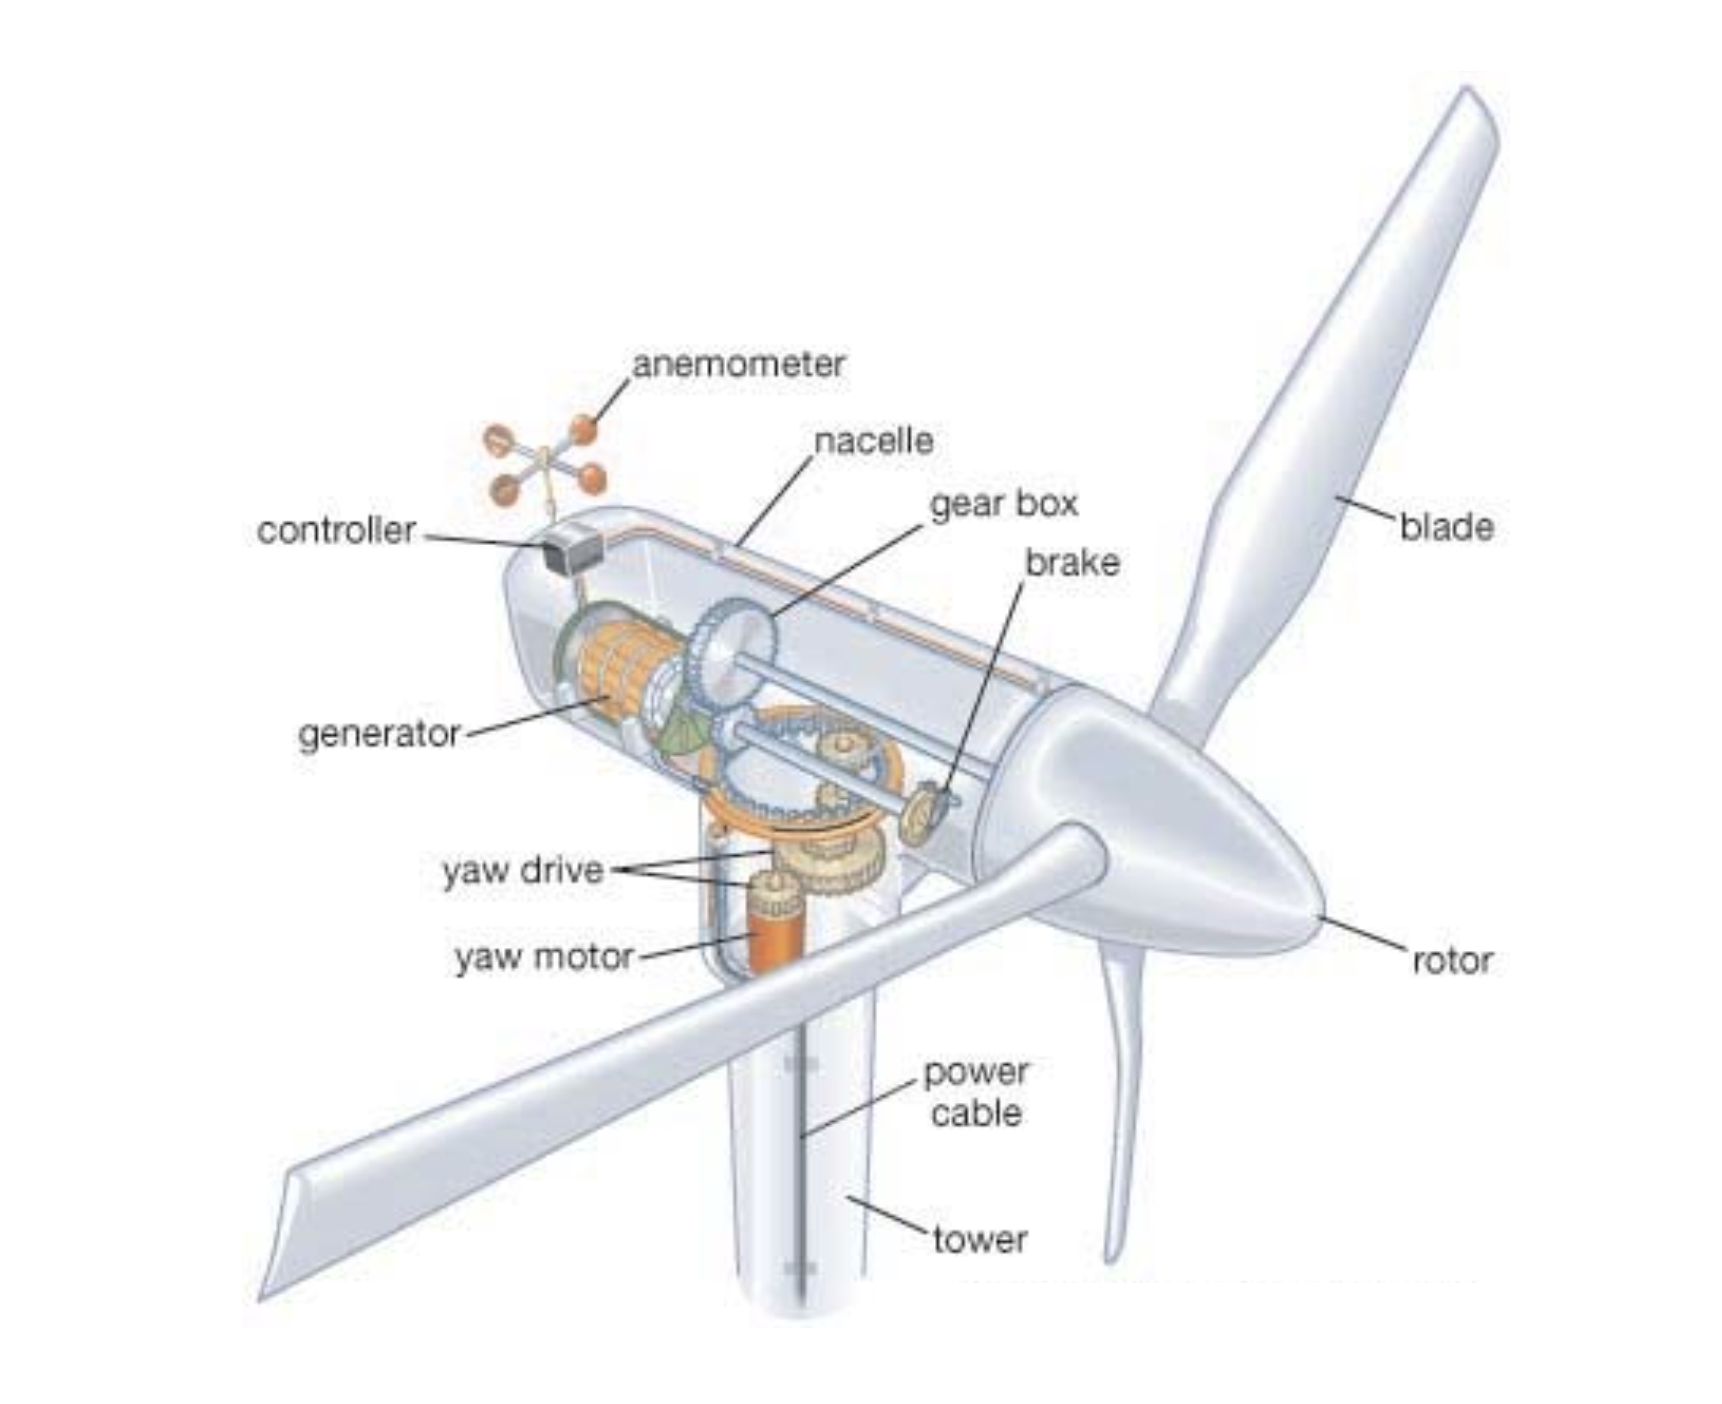
\includegraphics[width=1\linewidth]{fig/Simani_2015_process_diagram.png}}
%    
    \subcaptionbox{Control block diagram of a a wind turbine model \cite{Fragoso_et_al_2017}. Consisting of the input variables (left), the output variables (right), the controller (Multivariable control), the wind turbine itself and the wind as a disturbance. \label{fig:control_block_diagram} }[.45\textwidth]{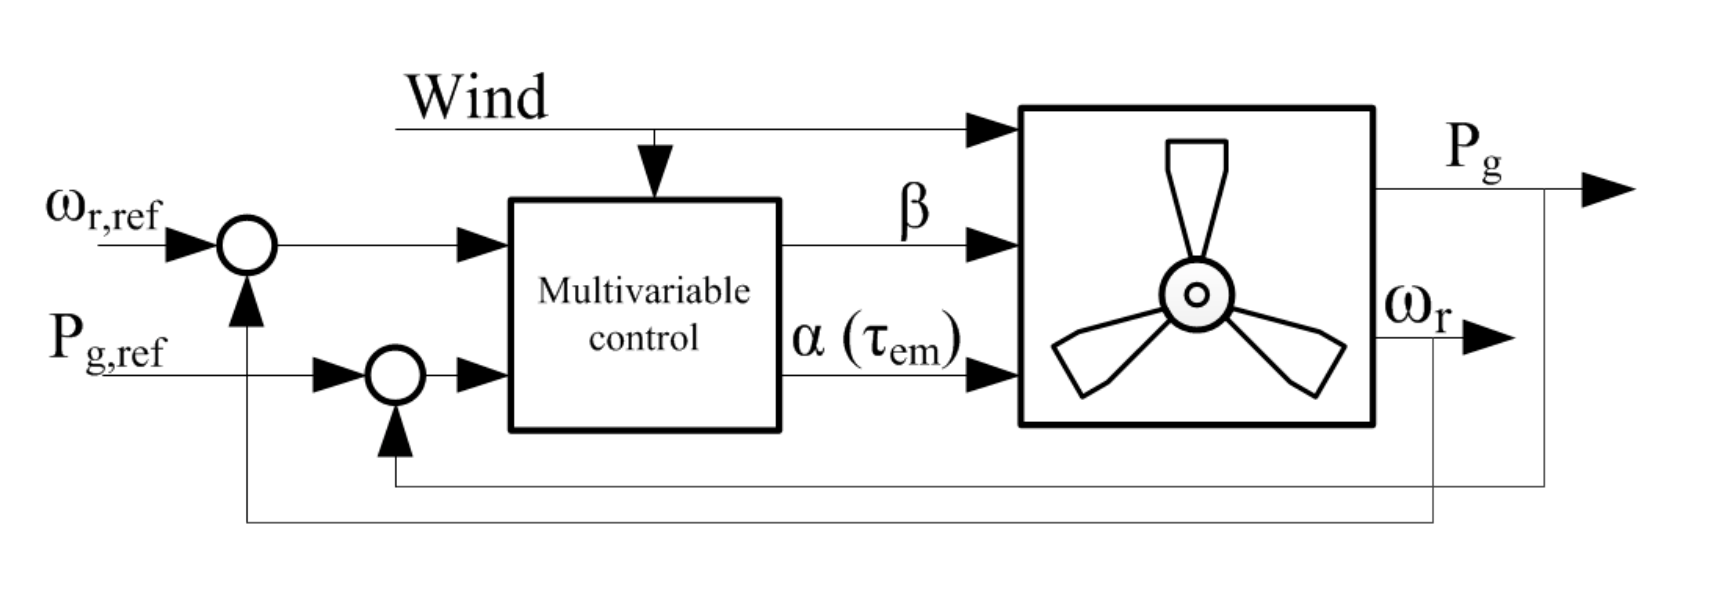
\includegraphics[width=1\linewidth]{fig/Fragaso_et_al_2017_process_scheme.png}}
%
    \caption{Comparison of a process diagram and the control block representation of a wind turbine.}
    \label{fig:compare_block_diagram_vs_process_diagram}
\end{figure}

\textbf{Control objective} Fragoso  et~al. discusing two different objective at two different operating states.
If the turbine is operated in partial load the objective is to maximize the power that can be captured from the wind.
The objective changes to maintaining the power constant at the rated power if the turbine is operated in full load.

\textbf{Input variables} Pitch angle $\beta$ and generator torque $\tau_{em}$ are commonly used as input variables. 

\textbf{Output variables} The rotational speed $\omega_r$ and generated electric power $P_G$ are the output variables of the system.

\textbf{Constraints} For controller design a linear model (derived by identification) is obtained by the authors. 
For further constraints Figure 13 and Figure 14 in Fragoso  et~al. publications are analyzed.
The following constraints can be seen in the output and control signals.

\begin{table}[H]
    \label{tab:constraints}
    \caption{Possible constraints for input and output variables.}
    \centering
    \begin{tabular}{ccccc} \toprule
            & $\omega_r \left[\text{rpm}\right]$ & $P_G \left[\si{\watt}\right]$ & $\beta \left[\si{\degree}\right]$ & $\alpha \left[\text{\%}\right]$ \\ \midrule
        Min & 1550 & 5 & 0  & 60 \\
        Max & 1750 & 7 & 25 & 75 \\ \bottomrule
    \end{tabular}
\end{table}


\textbf{Operating characteristics} The process is a continuous batch process.
The wind mill produces a laminar flow of air.
This is not the case in general.
If the stream of air is not laminar turbulences will occur at the blades.
This will introduces further disturbances which hard to calculate or estimate.

\textbf{Control structure}
The rotational speed $\omega_R$ and generated electric power $P_G$ are the controlled variables, blade pitch angle $\beta$ and the duty cycle $\alpha$ are the manipulated variables and the wind speed $v$ is counted as a disturbance.
The system is a multiple input multiple output (MIMO) system or two input and two output (TITO) system.
In total one $\text{H}_{\infty}$ based robust controller and three decoupling approaches are developed. 

\subsection{Model equation} \label{sec:intro:model_eq}

Fragoso et~al. defining their model through nonlinear ordinary differential equations. They distinguish between the electromechanical and electrical subsystems. Here only a brief overview is given. All relevant equations and parameter are published \cite{Fragoso_et_al_2017}.

For the mechanical subsystem the rotational speed $\omega_R$ is given by
\begin{align}
    J_t \frac{d\omega_r}{dt} = \tau_a - \tau_{em}
\end{align}
Here $J_t$ is the total inertia momentum of the system.
$\tau_{em}$ is the electromechanical torque and $ \tau_a$ the aerodynamic torque which can be expressed as a nonlinear function of wind speed $v$ and a power coefficient $C_p(\lambda ,\beta)$.
Where $\lambda$ is the tip speed ratio and $\beta$ the pitch angle.
Fragoso et~al. especially describe the power coefficient as an important parameter for the control and emphasises its nonlinear influence to the systems dynamics.


The electromechanical torque and the generated electrical power define the electrical subsystem.
\begin{align}
    \tau_{em} &= k_t i_g \label{eq:intro:tau_em}\\
    P_g &= \eta \tau_{em} \omega_r \label{eq:intro:P_g}
\end{align}
In both equations the efficiency is represented by $k_t$ and $\eta$ respectively for the electromechanical torque and the generator.


\subsection{Further reading}

\begin{figure}[htp]
    \centering

    \subcaptionbox{Process block diagram of a wind turbine with dynamics of field current and blade angles \cite{Adanez_et_al_2018}. \label{fig:Adanez_turbine_scheme}}[.3\textwidth]{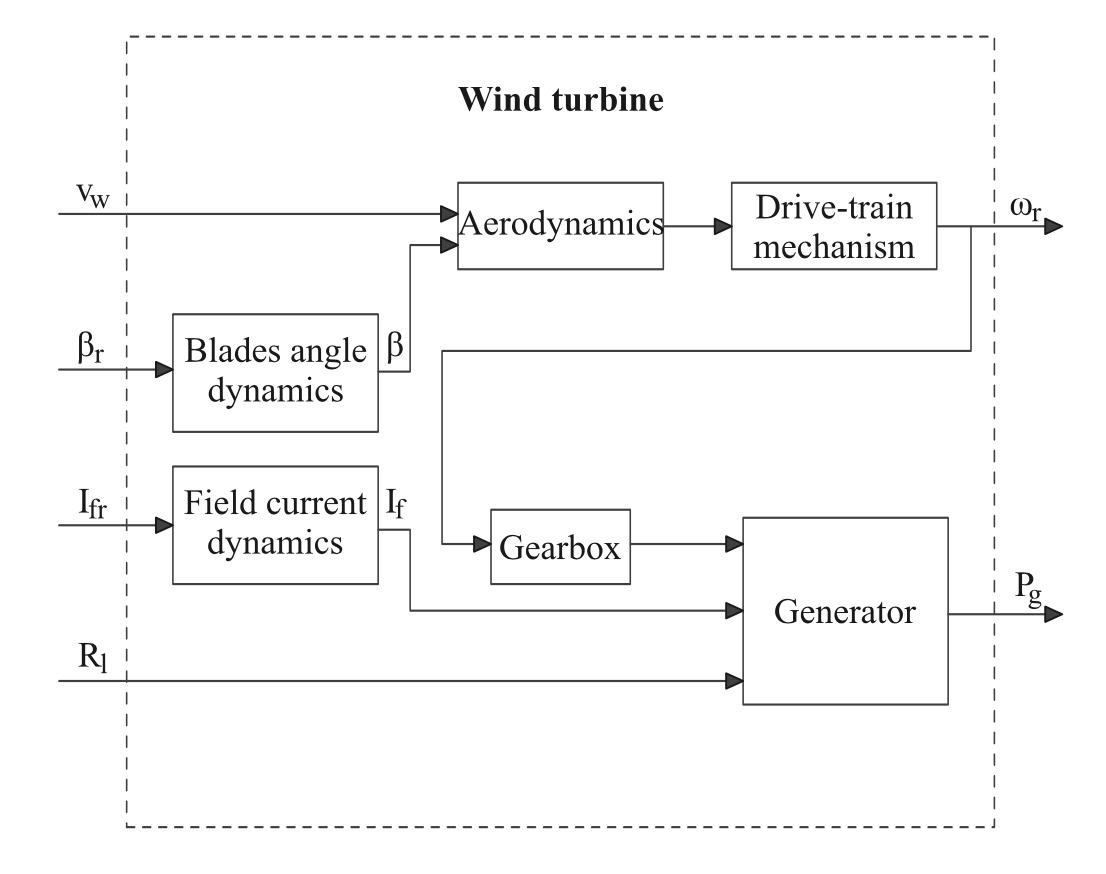
\includegraphics[width=1\linewidth]{fig/Adanez_et_al_2018_turbine_scheme.png}}
%
    \subcaptionbox{The control scheme used by Yuan, Cheng and Tang \cite{Yuan_Chen_Tang_2020}.  \label{fig:Yuan_Chen_Tang_control_scheme}}[.3\textwidth]{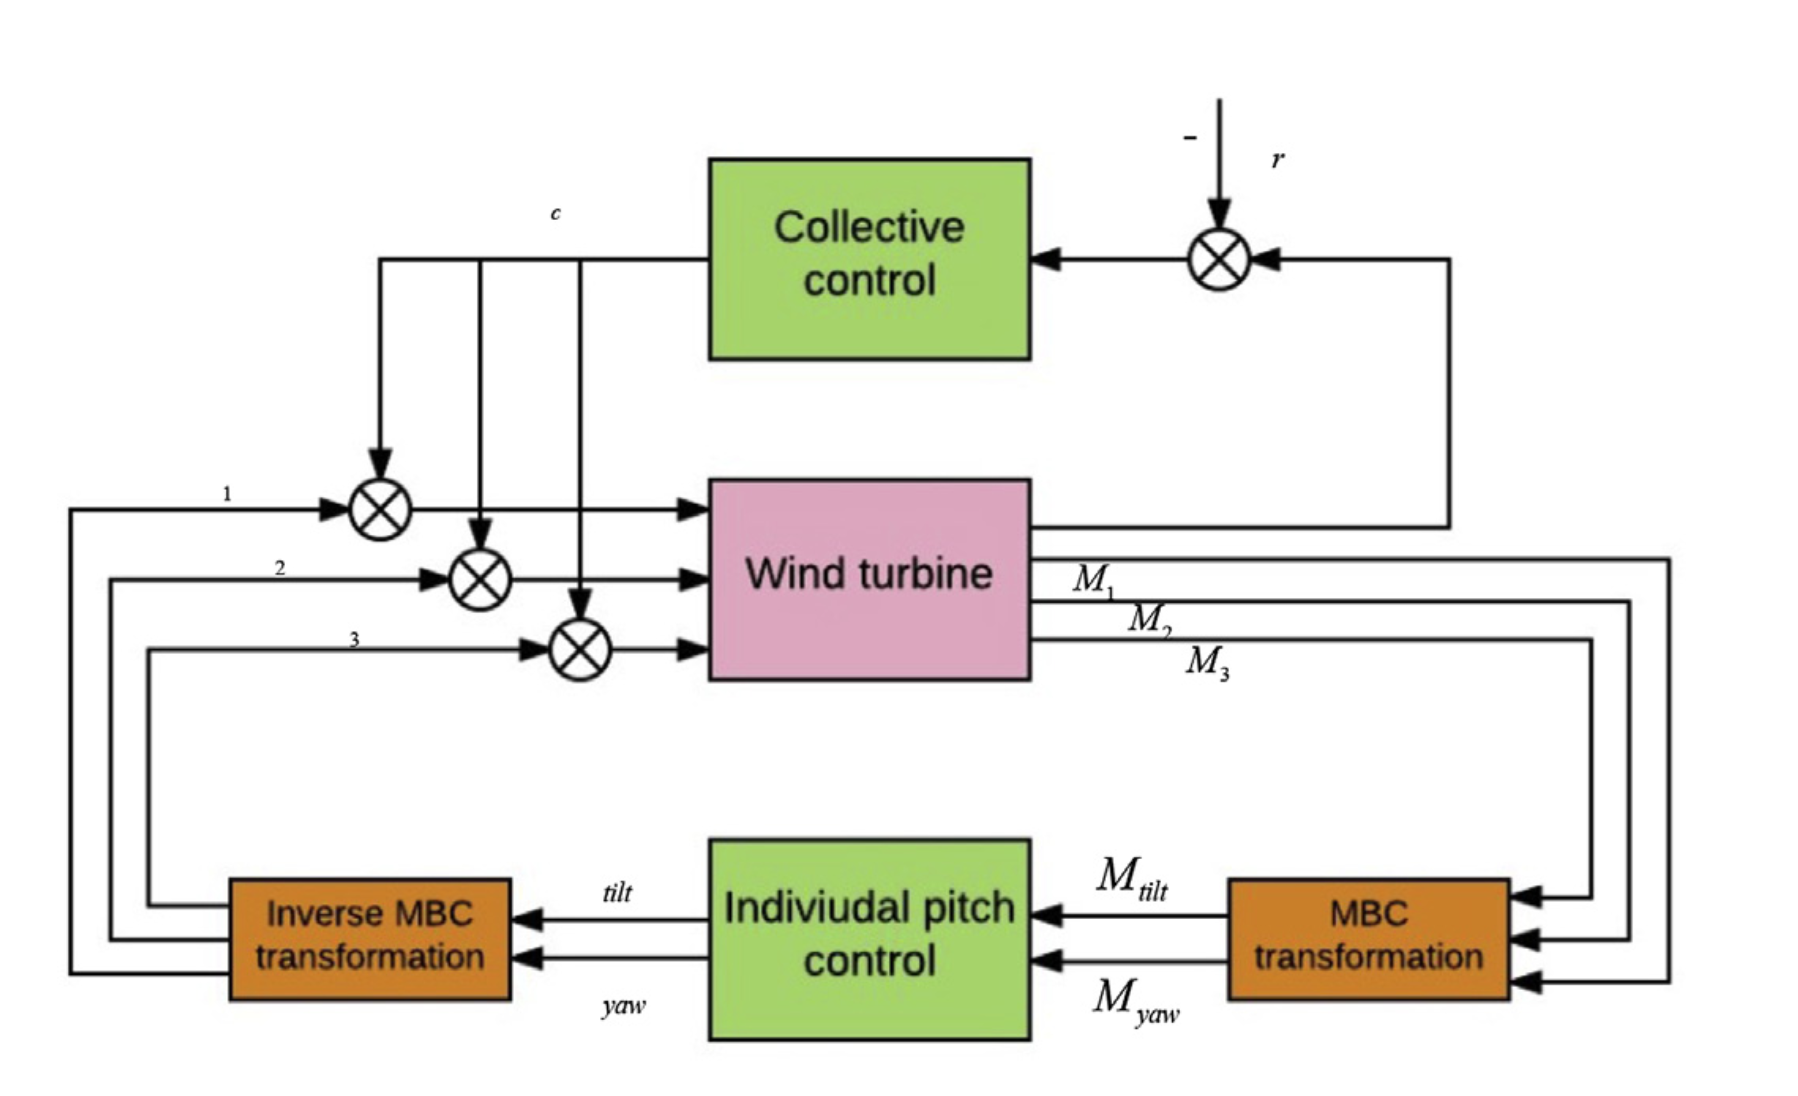
\includegraphics[width=1\linewidth]{fig/Yuan_Chen_Tang_2020_advanded_control.png}}
%
    \subcaptionbox{Visualization of switching control structures when wind turbine is in different operating conditions \cite{Simani_2015}.  \label{fig:Simani:switching_control}}[.3\textwidth]{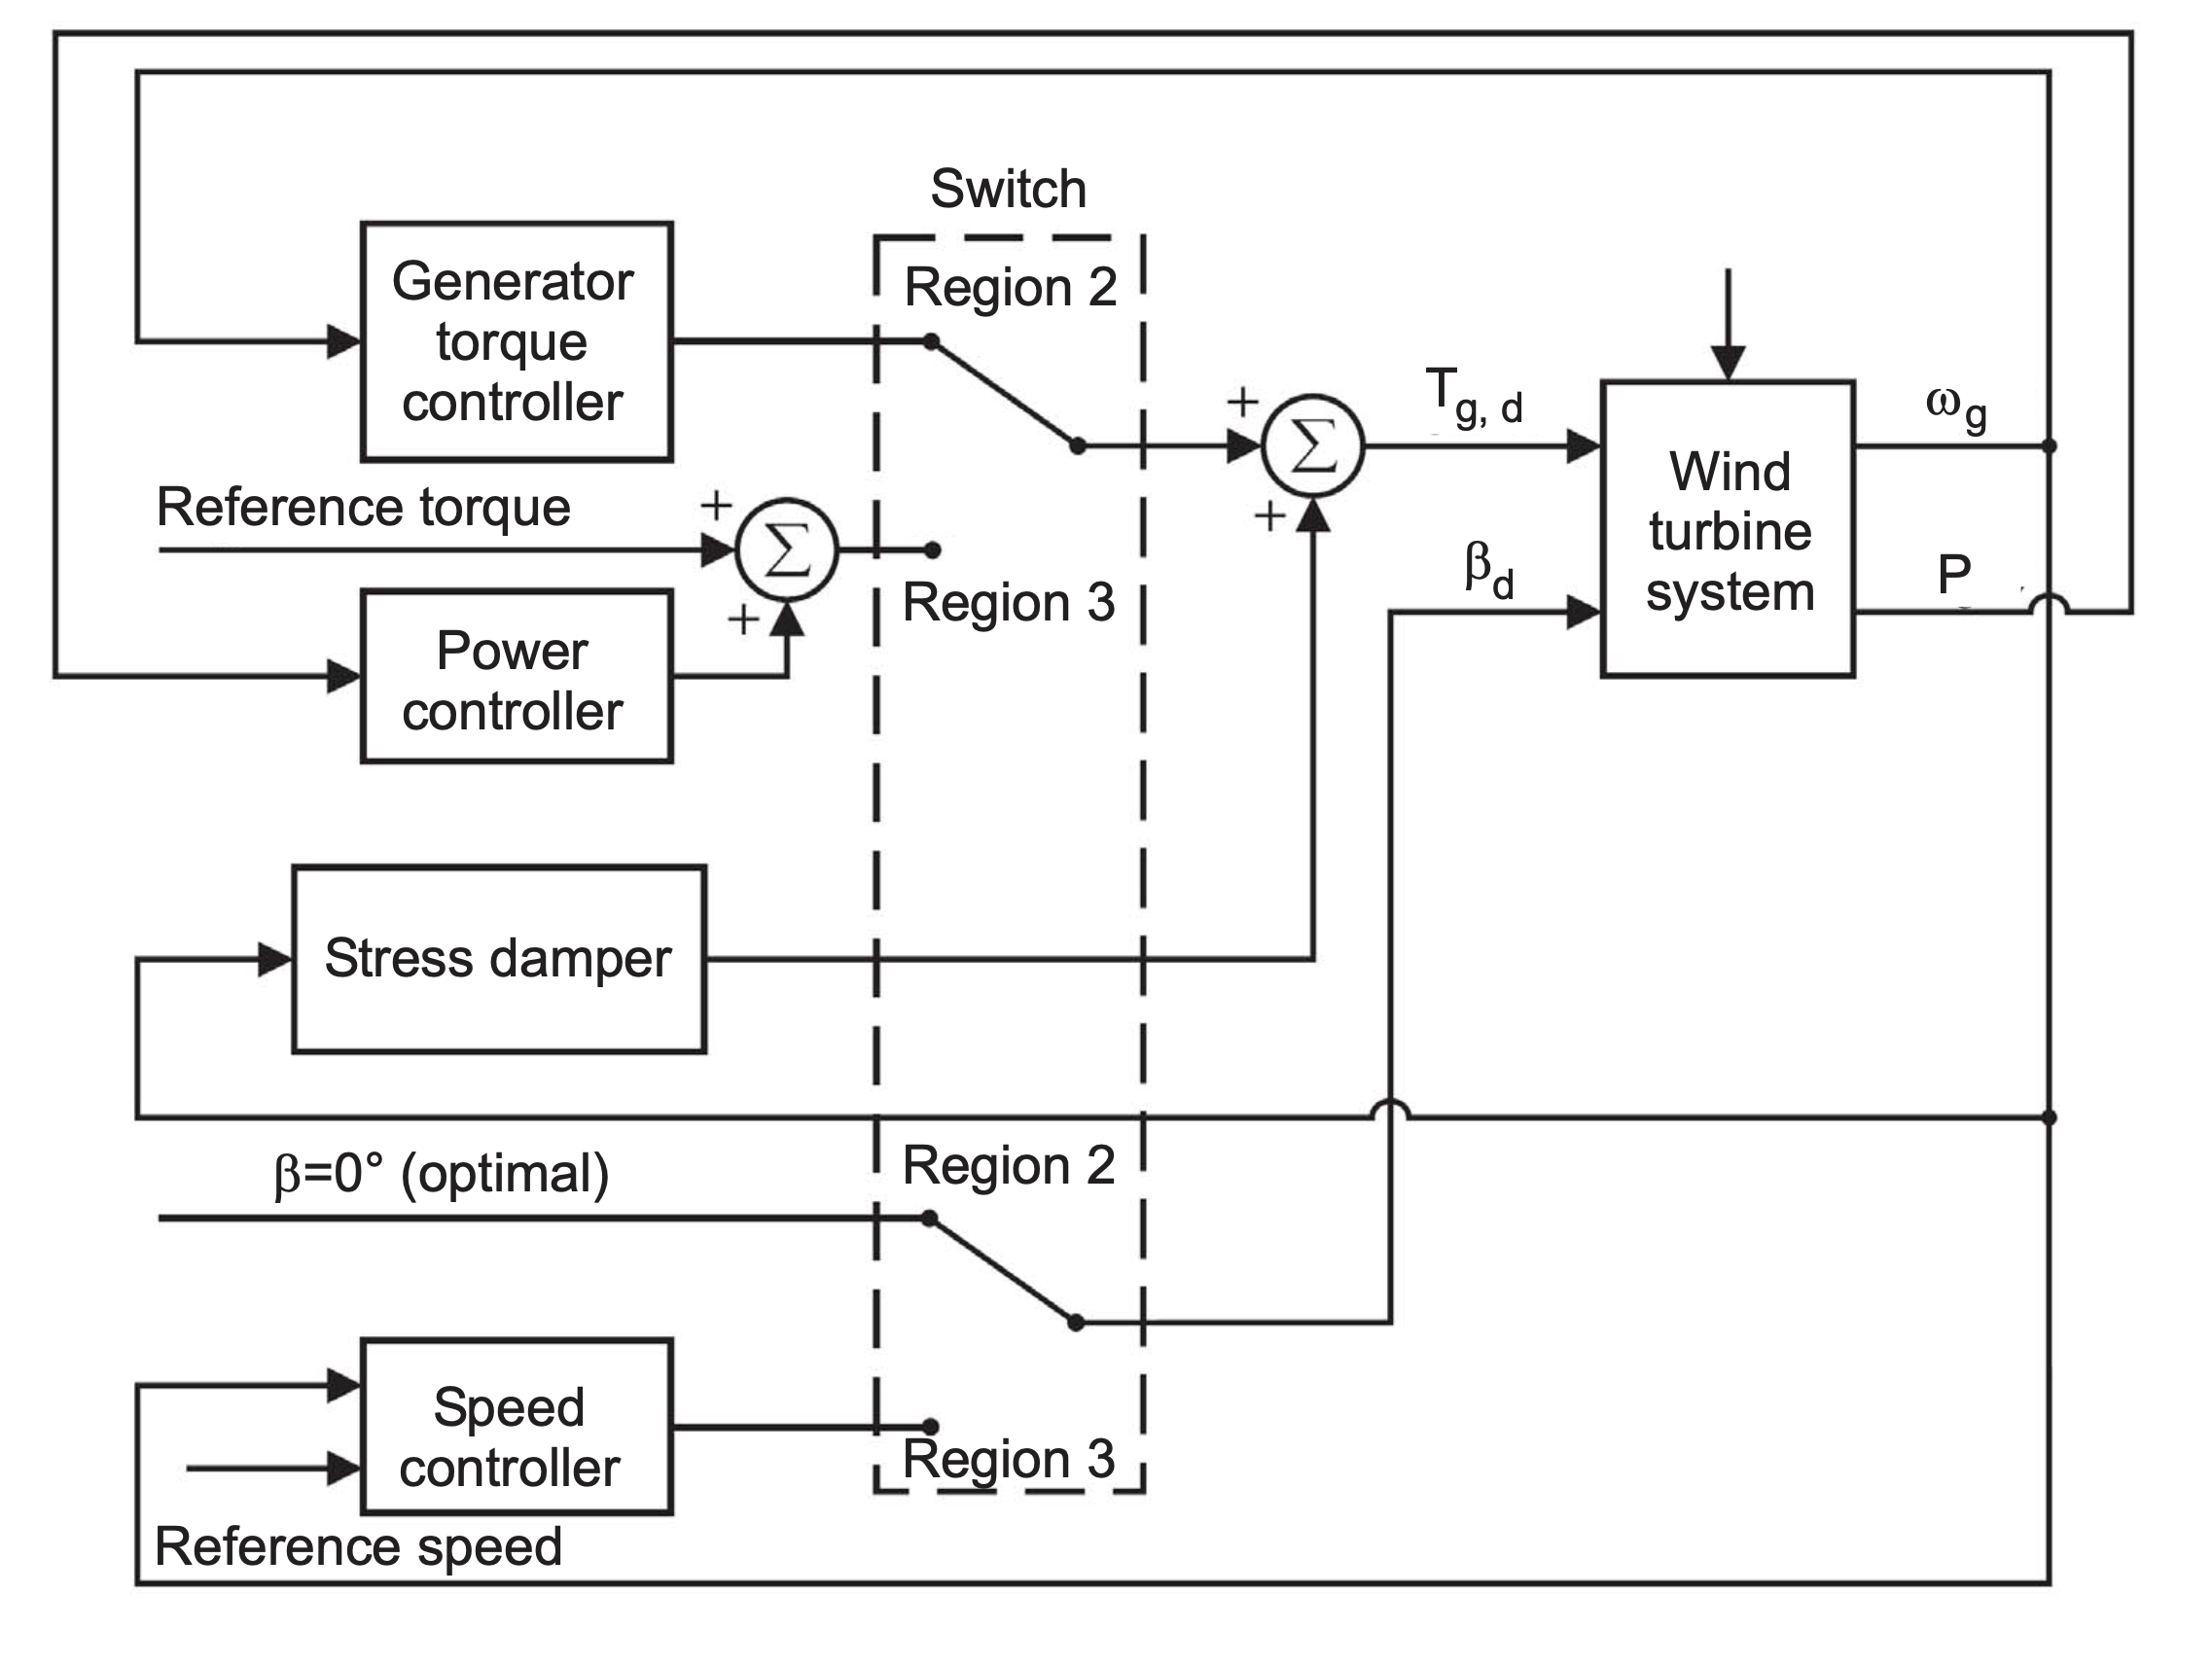
\includegraphics[width=1\linewidth]{fig/Simani_2015_switching_control.png}}
%
    \caption{Comparison of different visualization of control and system structures.}
    \label{fig:different_schemes_compared}
\end{figure}

Adánez et~al. published a control approach for a wind turbine based on incremental state model in 2018 \cite{Adanez_et_al_2018}.
The authors gave an overview over recent literature before describing their model of a wind turbine.
In comparison to Fragoso et~al. their schematics showing a more detailed look at the different parts of the system (\autoref{fig:Adanez_turbine_scheme}).
At the same time, however, it can be seen that very similar input and output variables are used.
They develope a multivariable discrete state model and an incremental state model. Besides that, an observer for the state feedback controller is derived.



Yuan, Cheng and Tang are describing in their work from 2020 the problems arising from the increasing blade sizes of modern wind turbines and thereby developing challenges in controller design \cite{Yuan_Chen_Tang_2020}.
In contrast to the aforementioned publication the authors do not show a scheme of the overall system, but instead providing a visual representation of the control structure (\autoref{fig:Yuan_Chen_Tang_control_scheme}).
The system itself is implemented in third party code and not as clearly shown as in the other publications.

Simani gives an full overview of the topic of modeling wind turbines \cite{Simani_2015}.
He summarizing not only models for the generator and blades but also for the wind turbine tower itself and the dynamics regarding blade motions.
In contrast to all other mentioned publication he is giving an overview of switching control structure when the turbine is in different operating conditions (\autoref{fig:Simani:switching_control}).
Also he is emphasising the switch in control objectives in different operating conditions.

\subsection{Summary}

The work of Fragoso et~al. seems to fit best in the criteria of the course by clearly naming all important design aspects and deriving comprehensible and probably easy to re-implement model.

\subsubsection{Simulating the model}

In Table 2 Fragoso et~al. published several transfer function for different wind speed.
These transfer function could be used to simulate the model.

For the ordinary differential equation all the  necessary parameters for a simulation seem to be given.
Also initial condition are formulated or could be read from Figure 13 and 14.

\section{System Analysis} \label{sec:analysis}

This section deals with the analysis of the aforementioned system of a wind turbine.
First, the description of the ODE system, which is insufficient for an implementation, is presented (\autoref{sec:analysis:ODE}) and the problems encountered are briefly described.

Second, the implementation of the system via transfer function is introduced \autoref{sec:analysis:tf}.
All important steps to implement the system in Matlab are shown.
By using figures published by Fragoso et al.– \cite{Fragoso_et_al_2017} the implementation in Matlab is verified.

The following chapter (\autoref{sec:condes}) is dealing with controller design. One important step of controller design is the relative gain array, which is conducted at the end of tis section.

\subsection{Simulation of ODE system} \label{sec:analysis:ODE}

Fragoso et al.~ \cite{Fragoso_et_al_2017} present a system of ODE for the wind turbine model.
As described in \autoref{sec:intro:model_eq} the model is subdivided into two parts.
The electrical subsystem is based in on two algebraic equations (\autoref{eq:intro:tau_em}, \autoref{eq:intro:P_g}).

For the mechanical part an ODE is given
\begin{align}
    J_t \frac{d \omega_t}{dt} = \tau_a - \tau_{em}, \label{eq:analysis:ODE_mechanical}
\end{align}
where $\tau_a$ is the aerodynamic torque and defined as
\begin{align}
    \tau_a = \frac{1}{2} \rho \pi R^3 \frac{C_p\left( \lambda, \beta\right)}{\lambda} v^2.
\end{align}
The power coefficient $C_p$ is only described by a figure (see Figure 4 in \cite{Fragoso_et_al_2017}).
In Fragosos work \cite[p. 54 ff.]{Fragoso_PhD_2016} a function for $C_p$ is derived and also a figure shows the global course of the function (see Figure 3.8, p. 56).
In this function nine heuristic parameters are used to determine the characteristics.
It is unclear if this function is also used in the work of Fragoso et al.~ or not.

In the appendix of Fragosos PhD-thesis there are tabulated value for $C_p$.
These were implemented as a lookuptable in Matlab.
By using the lookup table, values for $C_p$ could be determined, but the solutions of the ODE were not in a realistic range of values.

\begin{lstlisting}[style=Matlab-editor,caption={Matlab function for lookuptable. With this function we can get a corresponding $C_p$ value for given $\beta$ and $\lambda$. The \texttt{.csv}-file can be found in the GitHub repository under},captionpos=b,label={list:analysis:lookup}]
% Loading tabulated values as .csv file
p.lookup = readtable('lookuptable_c_p.csv');
% Setting corresponding column names 
p.lookup.Properties.VariableNames = {'wind_speed','rotor_speed','U','i_a','P_e','P_m','lambda','C_p','C_q','beta'};

% Looking up values for values of lambda and beta
function C_p = power_coefficient(lambda,beta,lookup)
    C_p = interp1(lookup.lambda(lookup.beta==beta),lookup.C_p(lookup.beta==beta),lambda);
end
\end{lstlisting}

Even if it is possible to get correct values for $C_p$, we still have only one ODE and a algebraic equation.
This is not representing a systems with two systems states.

Due to the problems mentioned here, the representation and solution of the system in state space was not pursued further and the transfer function mentioned in the Fragose et al.~ was used instead.

\subsection{Implementation of transfer function model} \label{sec:analysis:tf}

All controllers will be designed based on a linear model.
For different wind speeds $v$ Fragoso et al.~ identified five different linear models.
The pitch angel $\beta$ and the duty cycle $\alpha$ are the systems states.
The outputs are the rotational speed of the blade $\omega_r$ and the generated electric power $P_g$.
\begin{align}
    \begin{pmatrix}
        \omega_r \\
        P_g
      \end{pmatrix} = 
      G(s) 
      \begin{pmatrix}
        \beta \\
        \alpha
      \end{pmatrix} + G_D(s) v
\end{align}

The transferfunctions $G$ and $G_D$ where identified for windspeed $v=\left[6,7,8,9,10 \right] \si{\metre\per\second}$.
The results can be found in \cite[Table 2]{Fragoso_et_al_2017} and will not be reprinted here.

\begin{table}[H]
    \label{tab:analysis:import_var}
    \caption{Compilation of the most important variables, their meaning, unit and value range. The value ranges in italics are estimated values derived from figures. In addition, only the deviation $\Delta v$ is given, as we consider the disturbance in the following sections only as a deviation from zero. That is why we also consider a maximum value range between -1 and 1, as we would enter the \textit{domain} of another transfer function for larger values.}
    \centering
    \begin{tabular}{cllcc} \toprule
        Variable & Name & Interpration & Unit & Range \\ \midrule
        $\Delta v$ & change in windspeed & disturbance  & \si{\metre\per\second} & $\mathit{\left[-1,1\right]}$\\
        $\beta$ & pitch angle & state & \si{\degree}& $\left[0,25\right]$ \\
        $\alpha$ & duty cycle& state & 1 & $\left[0,1\right]$\\
        $\omega_r$ & rotational speed of blade & input & rpm & $\mathit{\left[1400,2000 \right]}$  \\
        $P_g$ &generated electric power &input & \si{\watt} &  $\mathit{\left[3,9 \right]}$\\ \bottomrule
    \end{tabular}
    \label{tab:analysis:constraints}
\end{table}

\subsubsection*{Implementation in Matlab}

To generate the transfer functions in Matlab the \texttt{tf}-command and the \texttt{table} function are used.

\begin{lstlisting}[style=Matlab-editor,caption={},captionpos=b,label={list:analysis:tf}]
% Wind speed: 6 m/s
G_S_num_6 = {-8.059,-405.4;-0.0081479,4.4195};
G_S_denom_6 = {[75.27,17.35,1],[28.25, 16.47, 1];[0, 16.873, 1],[0, 1.7589, 1]};
G_D_num_6 = {364.9; 1.139};
G_D_denom_6 = {[118.3, 21.76, 1];[65.28, 17.09, 1]};

... Wind speeds 7,8,9 an 10 m/s ...

% Making a table to store all transfer_function
varNames = ["wind_speed","G_S_numerator","G_S_denominator","G_D_numerator","G_D_denominator","G_S","G_D","RGA"];
table_tf = table;
% Naming the columns in the table
table_tf.Properties.VariableNames = varNames;

% Filling the table with numerator and denominator
table_tf(1,1:5) = {6,G_S_num_6,G_S_denom_6,G_D_num_6,G_D_denom_6};
...
table_tf(5,1:5) = {10,G_S_num_10,G_S_denom_10,G_D_num_10,G_D_denom_10};
table_tf.Properties.VariableNames = varNames(1:5);

% For loop for creating transfer function by using tf-command
for i = 1:5
    table_tf{i,6} = {tf(table_tf{i,"G_S_numerator"}{:},table_tf{i,"G_S_denominator"}{:})};
    table_tf{i,7} = {tf(table_tf{i,"G_D_numerator"}{:},table_tf{i,"G_D_denominator"}{:})};
    table_tf{i,8} = {NaN};
end
\end{lstlisting}

For each transfer function modeling the system behaviour for different wind speeds we have a numerator and denominator for the systems transfer function $G$ and the disturbance system $G_D$.
Those are stored as arrays \texttt{G\_num\_6}, \texttt{G\_D\_denom\_6}, etc.~, where the 6 at the end depicting the transfer function for a wind speed of $\SI{6}{\metre \per \second}$.

In line 17 ff. the numerator and denominator of all transfer function are stored in the table initialized in line 12.
Using the \texttt{tf}-command inside a \texttt{for-loop} (line 23 ff.) the transfer function is defined.
In line 14 every column of the table gets a name.

\subsubsection{Verifying the implementation}

The goal of verification is the recreation of relative step responses shown by Fragoso et al.~(\autoref{fig:analysis:fig_step_response}).
The figure is used as a benchmark.
If the global course of the step response can be readjusted, then one can assume that the model is implemented correctly.

\begin{figure}[H]
    \center
    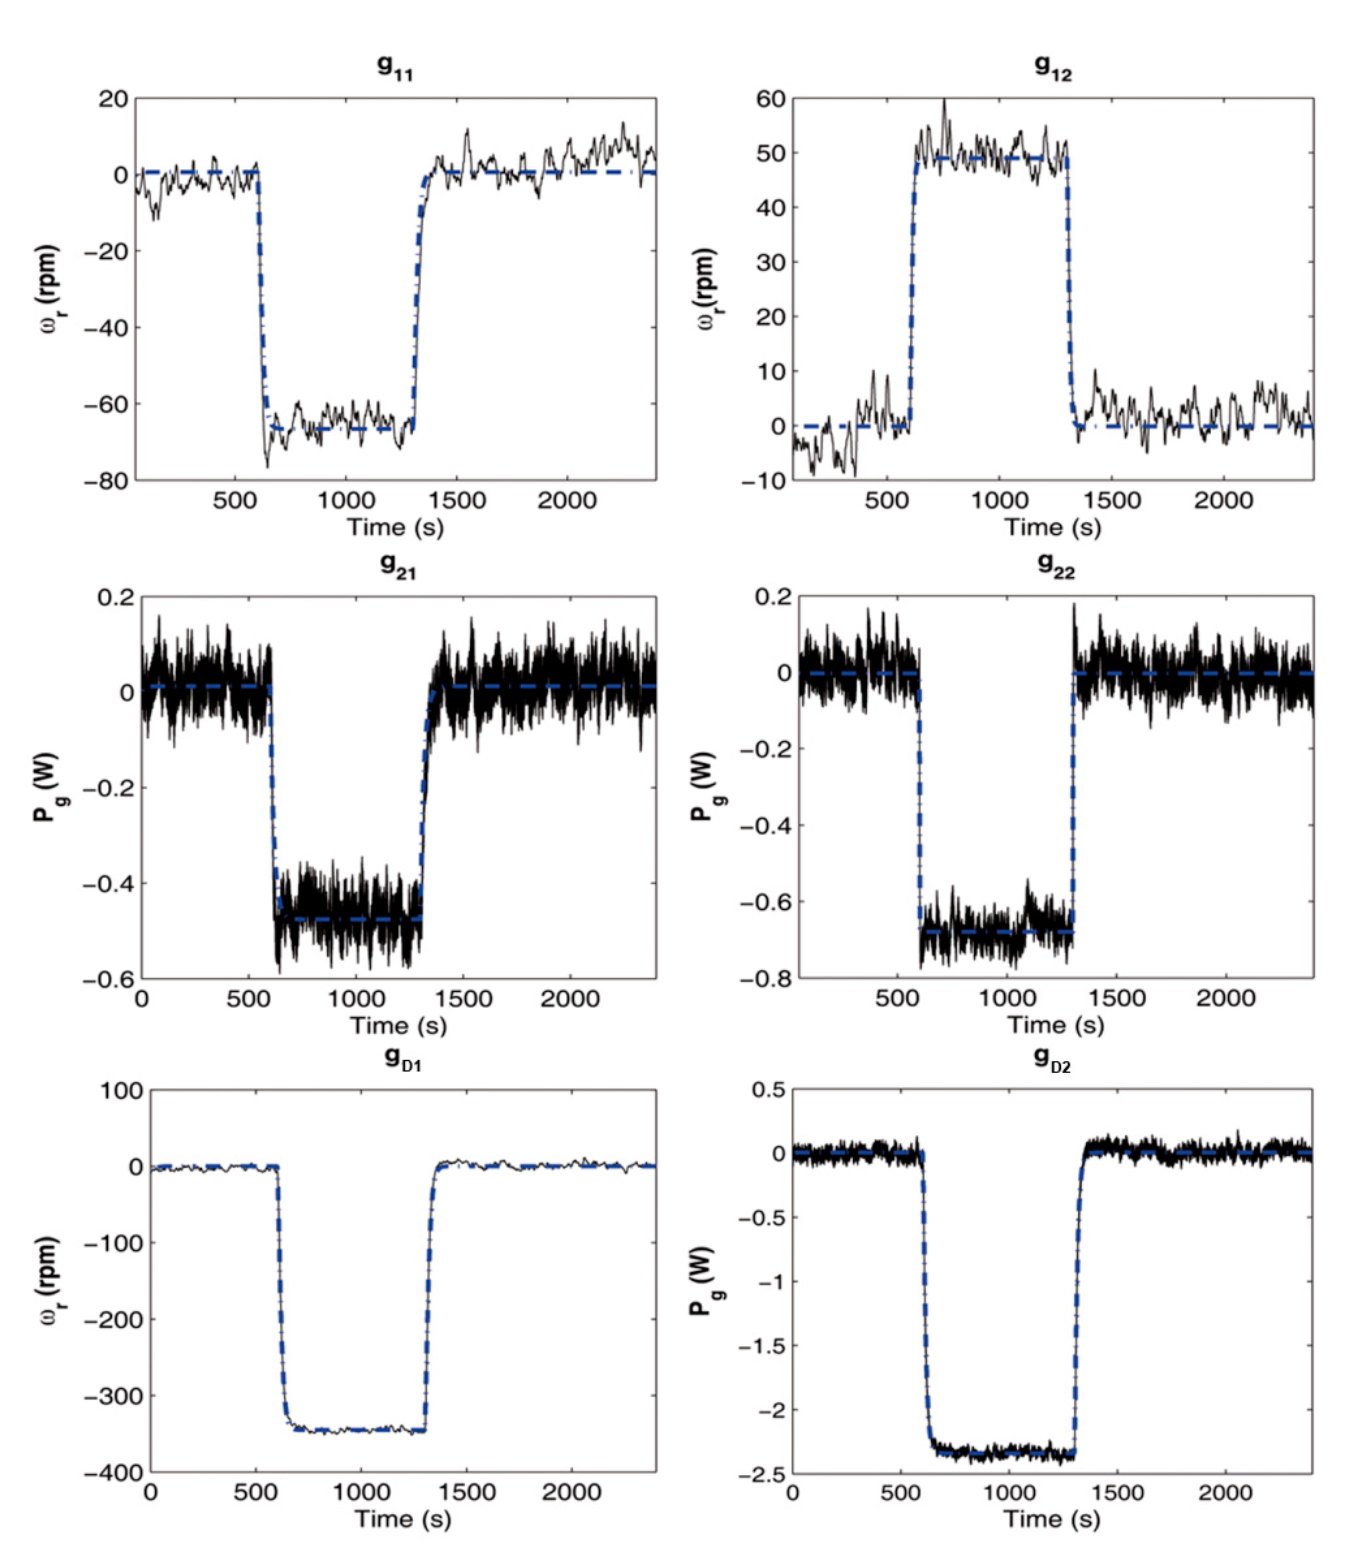
\includegraphics[scale=0.5]{fig/Fragoso_et_al_2017_fig6.png}
    \caption{The figure presented by \cite{Fragoso_et_al_2017} shows the relative step response of the identified system (dashed line) and the real system (solid) line.}
    \label{fig:analysis:fig_step_response}
\end{figure}

The six figures are labeled as $g_{ij}$ as changing input $i$ and showing the influence on output $j$.
The bottom two are referring to the influence of disturbance changes (changes in wind speed) when inputs are changed.
Unfortunately the exact values are not given in the paper and therefore must be reverse engineered.

\begin{table}[H]
    \caption{The tables shows the influence of an input to a single output. The table can be seen as an other way of displaying the results from \autoref{fig:analysis:fig_step_response}.}
    \centering
    \begin{tabular}{ccccc} \toprule
        Figure & Input & $\Delta$ & Output & $\Delta$ \\ \midrule
        $g_{11}$ & $\beta$    & \SI{7}{\degree}               & $\omega_r$  & $\SI{-70}{rpm}$ \\
        $g_{12}$ & $\alpha$   & $-0.1$                        & $\omega_r$  & $\SI{50}{rpm}$ \\
        $g_{21}$ & $\beta$    & \SI{12}{\degree}              & $P_g$       & $\SI{-0.5}{\watt}$ \\
        $g_{22}$ & $\alpha$   & $-0.1$                        & $P_g$       & $\SI{-0.7}{\watt}$ \\
        $g_{D1}$ & $v_{wind}$ & $\SI{-1}{\metre\per\second}$  & $\omega_r$  & $\SI{-300}{rpm}$ \\
        $g_{D2}$ & $v_{wind}$ & $\SI{-2}{\metre\per\second}$  & $P_g$       & $\SI{-2.3}{\watt}$ \\ \bottomrule
    \end{tabular}
    \label{tab:analysis:changes}
\end{table}

From left to right the first row of \autoref{tab:analysis:changes} can be read as: For figure $g_{11}$ the input $\beta$ is changed by \SI{7}{\degree} and will result in reducing the rotational speed $\omega_r$ by \SI{70}{rpm}.
All six figures presented by Fragaso et al.~ can be recreated by the values given in \autoref{tab:analysis:changes}.
\autoref{fig:analysis:recreate_step_changes} is one example representing the subfigure $g_{11}$ and using the values of the first row.

\begin{figure}[h!]
    \center
    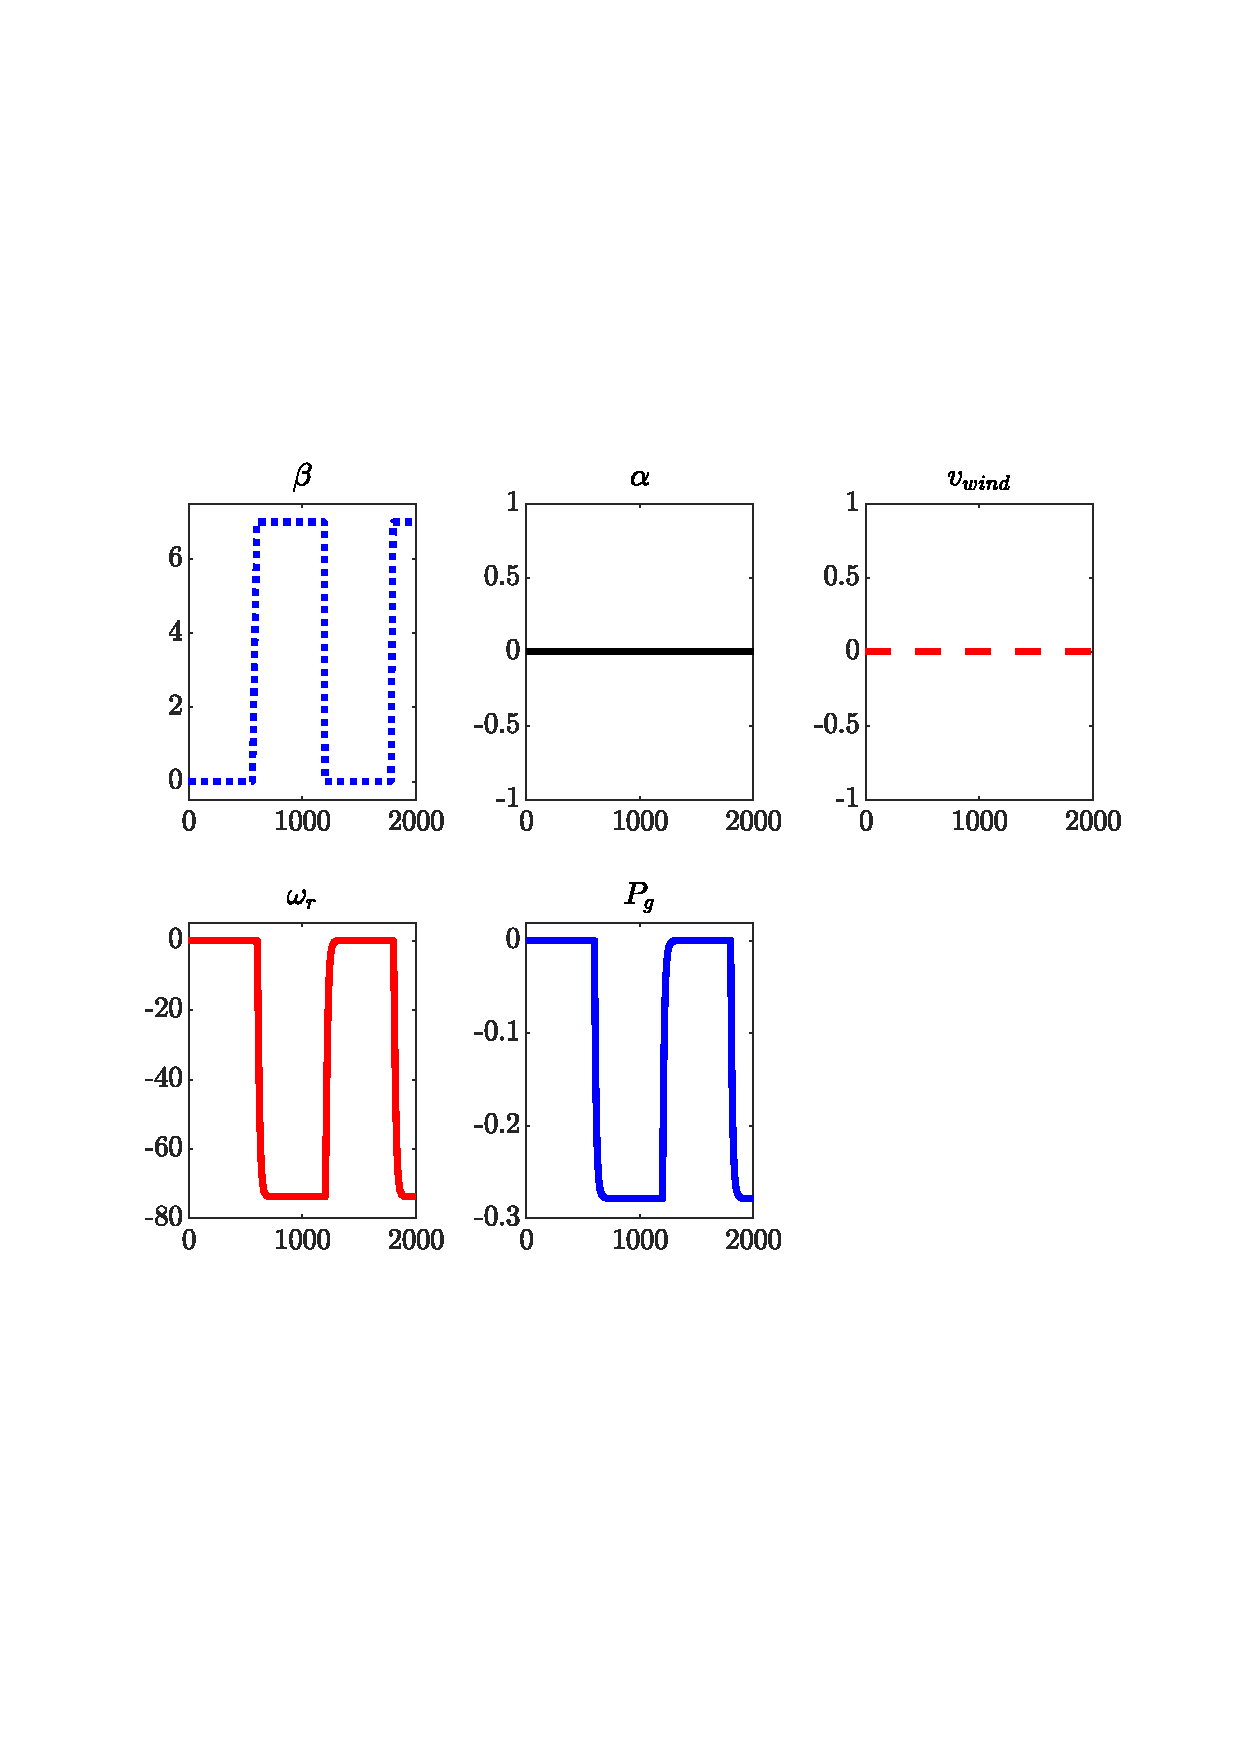
\includegraphics[scale=0.7,trim=60 200 50 150,clip]{fig/recreate_step_changes.pdf}
    \caption{Recreating subfigure $g_{11}$ by plotting inputs, outputs and the disturbance over time. A pulse with a period of \SI{1200}{\second} and a pulse width of \SI{600}{\second} changes $\beta$ by \SI{7}{\degree}. This results in reducing the rotational speed $\omega_r$ by \SI{70}{rpm}.}
    \label{fig:analysis:recreate_step_changes}
\end{figure}



\subsection{Relative Gain Array}  \label{sec:analysis:RGA}

The relative gain array is used to obtain a measure of the dependencies of inputs and outputs for a MIMO-system.
In this particular example we want to know the influence of rotational speed $\omega_r$ and the electrical power $P_g$ on pitch angle $\beta$ and duty cycle $\alpha$.


The RGA-matrix is symmetric and all column- and row-sums a equal to one.
For a $2\times2$-matrix we only need to calculate the element $(1,1)$ and deduce all other values.
\begin{align}
    \Lambda_{RGA} &= \begin{pmatrix}
        \lambda_{11} & \lambda_{12} \\
        \lambda_{21} & \lambda_{22}
    \end{pmatrix}, \text{with} \\
    & \lambda_{12} = \lambda_{21} \\
    & \lambda_{11} + \lambda_{12} = 1 \\
    & \lambda_{21} + \lambda_{22} = 1
\end{align}


\subsubsection*{Implementation in Matlab}


\begin{lstlisting}[style=Matlab-editor,caption={This Matlab function calculates a $2\times2$-RGA-matrix},captionpos=b,label={list:analysis:RGA}]
    function RGA = calculate_RGA(G_S_numerator)
        % Computation of RGA
        lambda_11 = G_S_numerator{1,1}/(G_S_numerator{1,1} - (G_S_numerator{1,2}*G_S_numerator{2,1})/G_S_numerator{2,2} );
        RGA = [[lambda_11, 1-lambda_11];[1-lambda_11,lambda_11]];
    end
\end{lstlisting}
    
In line four the RGA-matrix is calculated.
As previously described we only need to calculate  $\lambda_{11}$ and can deduce all other elements of $\Lambda$.

    

\subsubsection*{Results of RGA}

The investigation of the RGA for different wind speeds provides clearly different dependencies between the inputs and states.
The results are shown in \autoref{fig:analysis:RGA_results}.

\begin{figure}[H]
    \center
    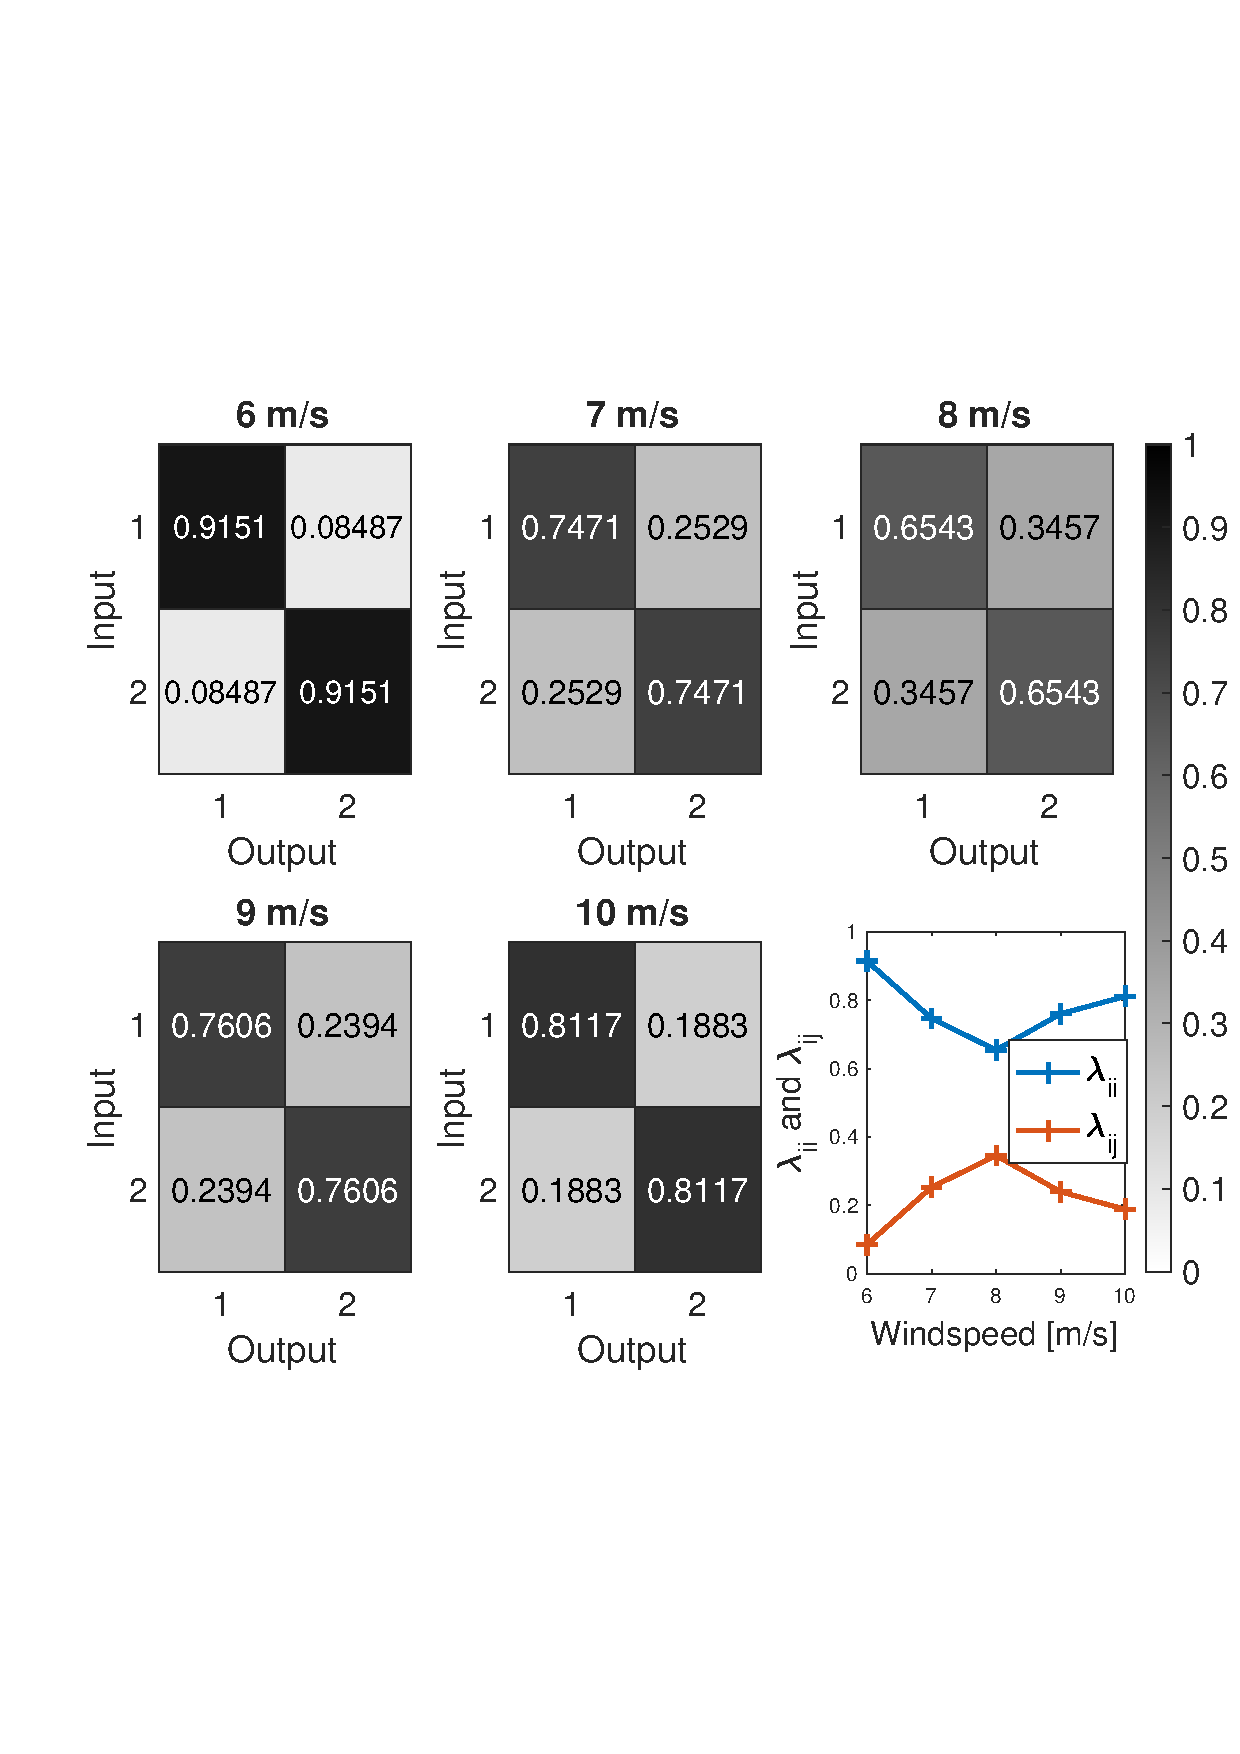
\includegraphics[scale=0.6,trim=40 180 0 120,clip]{fig/RGA_results.pdf}
    \caption{Visualization of the five RGA-matrices and a line plot for $\lambda_{ii}$ and $\lambda_{ij}$.}
    \label{fig:analysis:RGA_results}
\end{figure}

For very low windspeeds ($\SI{6}{\metre\per\second}$) the system is nearly decoupled.
At a windspeed of $\SI{10}{\metre\per\second}$, the system can also be considered almost decoupled.
If the the windspeed is approaching $\SI{8}{\metre\per\second}$ the peak coupling is reached.
This behaviour can be best seen at the line plot.
Both lines almost touch at a windspeed of $\SI{8}{\metre\per\second}$ and diverge before and after.

The results achieved are congruent with the findings of Fragaso et al. (\cite[p. 7]{Fragoso_et_al_2017}, \cite[p. 123]{Fragoso_PhD_2016})

In the following chapter we will design a controller for the \textit{hardest} condition of a coupled system with windspeeds of $\SI{8}{\metre\per\second}$.

\section{Controller Design} \label{sec:condes}

In the previous sections only the open loop behaviour is analyzed.
This section focuses on the controller design and closing the loop.
Therefore, this section describes the implementation of open and closed loop systems in Simulink (\autoref{sec:condes:implementation_simulink})

Two different techniques for controller design are described.
First, the Ziegler-Nichols method is shown (\autoref{sec:condes:ZN}).
For this method, two different approximations for the required \textbf{f}irst-\textbf{o}rder-\textbf{p}lus-\textbf{t}ime-\textbf{d}elay transfer function (FOPTD) are used.
The max-slope method (\autoref{sec:condes:ZN:maxS}) uses the inflection point of the step resoponse to determine the control parameters.
In contrast, the two-point method (\autoref{sec:condes:ZN:2p}) does not use derivatives, instead the points in time at which the step response has risen to 28\% or 63\% of its maximum value.
As a result, the method is also considered to be numerically more stable.

Second, the T-sum method (\autoref{sec:condes:Tsum}) is used to determine control parameters for a PID controller.
Here, the parameters are estimated by using the area under the step response.

\begin{figure}[H]
    \centering

    \subcaptionbox{Max-slope approximation\cite[Lecture 6, slide 12]{Dissli_Kienle_2023} \label{fig:condes:different_methods_maxSlope}}[.45\textwidth]{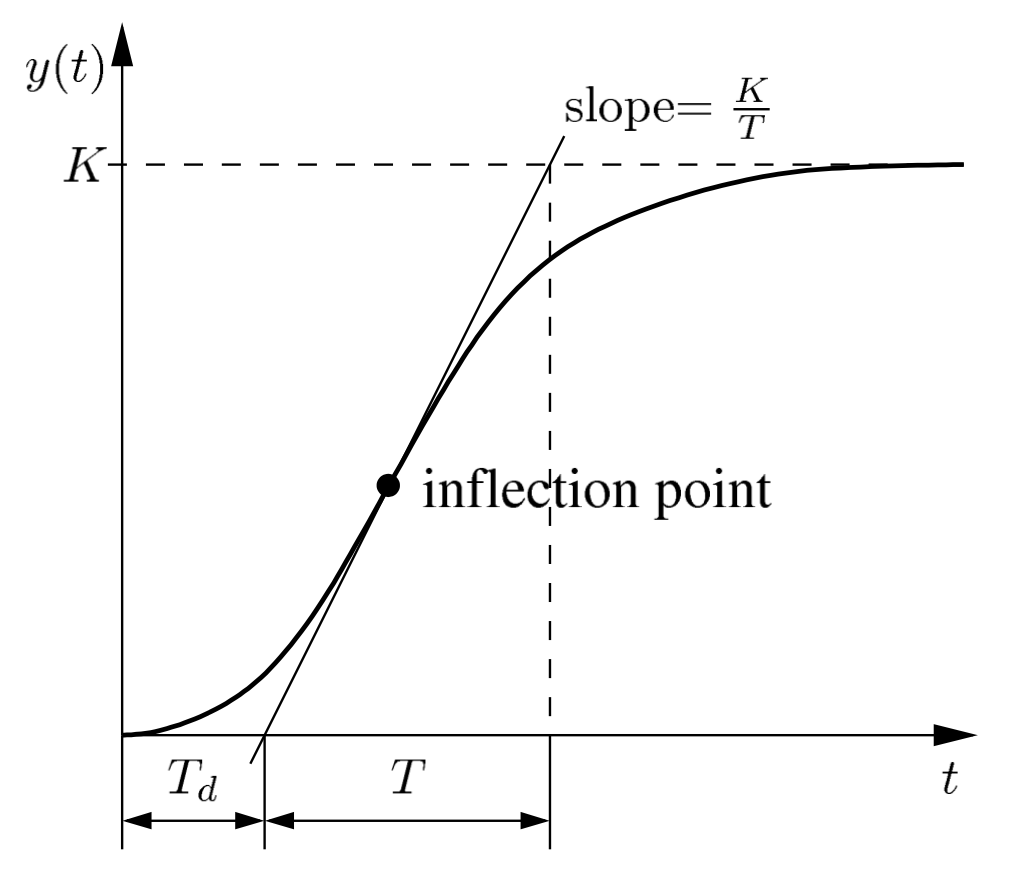
\includegraphics[width=1\linewidth]{fig/Dissli_Kienle_max_slope_2023.png}}
%
    \subcaptionbox{T-sum method \cite[Lecture 6, slide 17]{Dissli_Kienle_2023} \label{fig:condes:different_methods_Tsum}}[.45\textwidth]{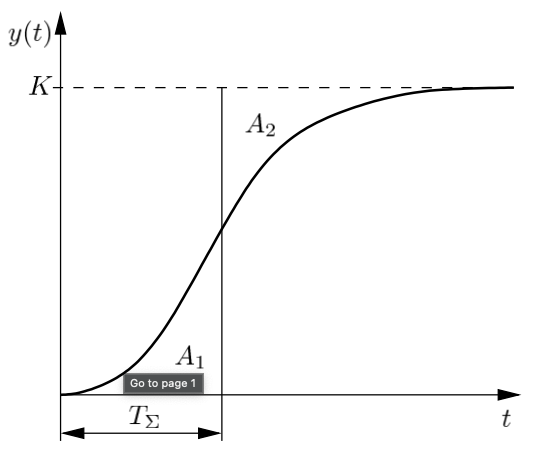
\includegraphics[width=1\linewidth]{fig/Dissli_Kienle_T_sum_2023.png}}
\\
\subcaptionbox{Two-point approximation \cite[Lecture 4, slide 6]{Dissli_Kienle_2023}  \label{fig:condes:different_methods_2p}}[.7\textwidth]{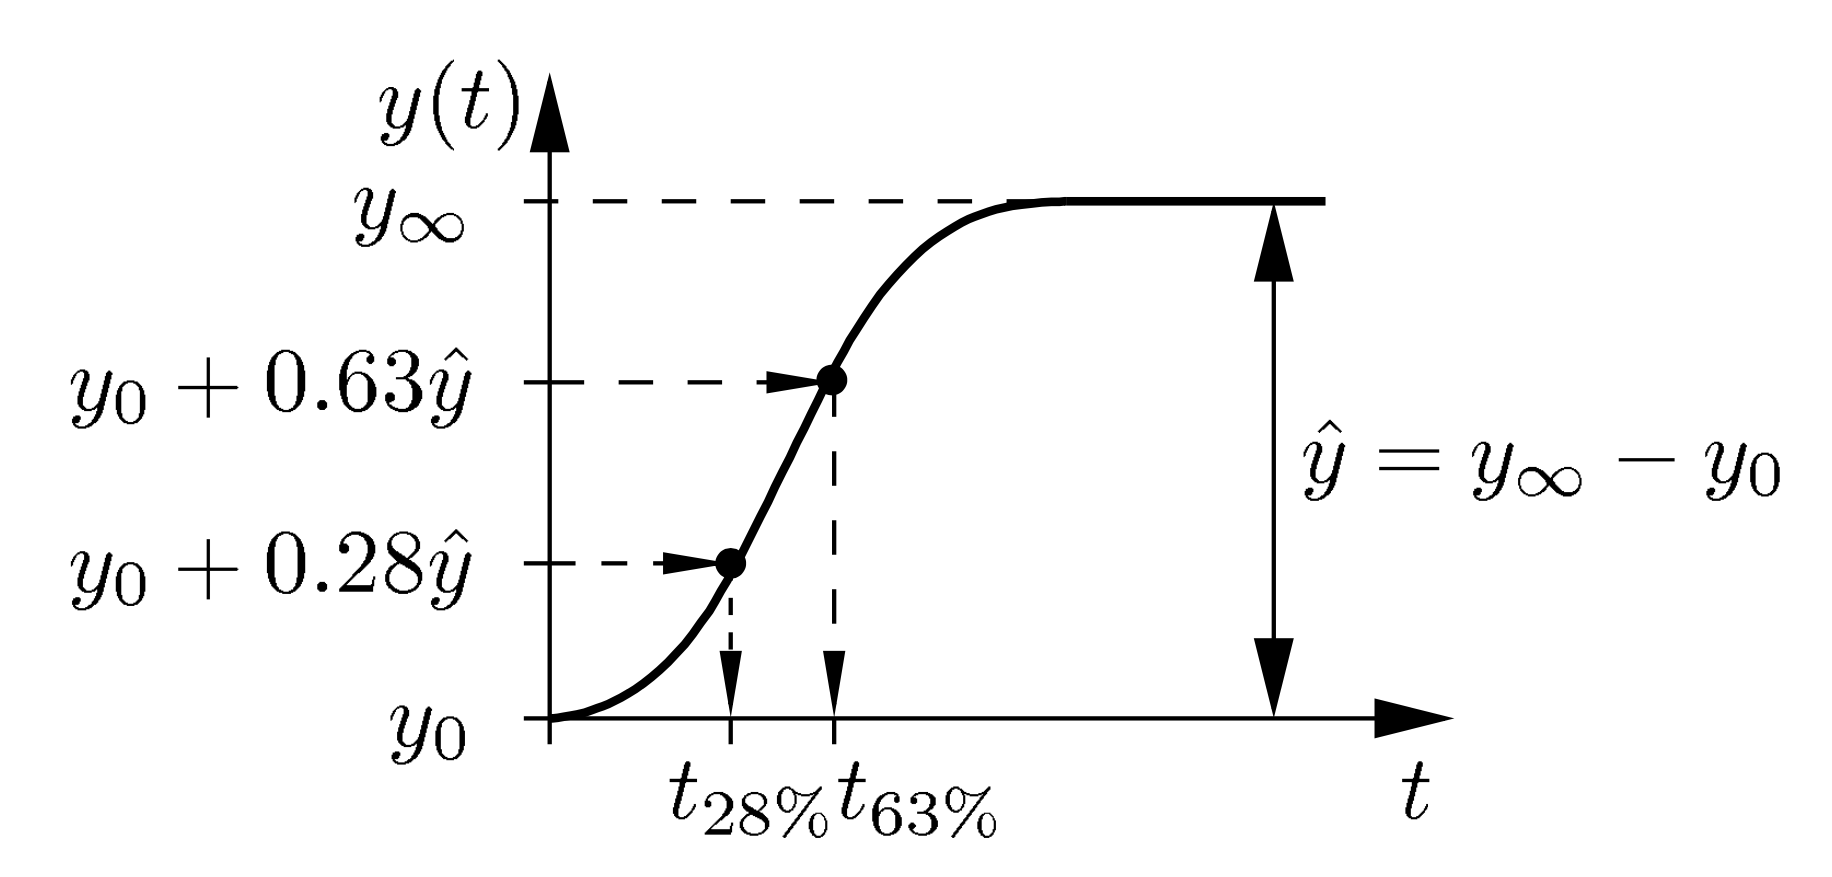
\includegraphics[width=1\linewidth]{fig/Dissli_Kienle_two_point_2023.png}}
    \caption{Visualization of two different approximation methods for Ziegler-Nichols controller design and the T-sum method for control parameter estimation. All plots from \cite{Dissli_Kienle_2023}}
    \label{fig:condes:different_methods}
\end{figure}


%Third, the relay-feedback method (\autoref{sec:condes:Relayfeedback}) as an example of an auto-tuning methods characterizes the control parameters.

In the end all methods are discussed and the robustness of some methods is shown (\autoref{sec:condes:discussion}).



\subsection{Ziegler-Nichols open loop method}\label{sec:condes:ZN}

The Ziegler-Nichols open loop method assumes an s-shape step response or an underlying first-order-plus-time-delay transfer function, respectively.
Looking at the given transfer function by Fragoso et~al. (\cite[Table 2]{Fragoso_et_al_2017}), we do not have this behaviour.
Therefore, we need to approximate a FOPTD transfer function.
This can be done with two different approaches.
First, the max-slope approximation is used for controller design and second, the two-point method determines the controller's parameters.

In the following two subsection both methods and their Matlab implementation is discussed. 


\subsubsection{Max-slope approximation} \label{sec:condes:ZN:maxS}

The max-slope method focuses around the inflection point of the unit step response.

\begin{lstlisting}[style=Matlab-editor,caption={This code snippet show the general way of calculating the control parameters with the max-slope method.},captionpos=b,label={list:condes:maxS}]
[y,t_out] = step(G,t_linspace);
[slope, intcpt] = calc_infliction_point_slope(y,t_out);
tngt = slope*t_out + intcpt;
[K, T, T_d, t_inter] = calc_gain_time_const_time_delay(y,t_out,tngt);
\end{lstlisting}

In line 1 the step response of a transfer function \texttt{G} with the Matlab built-in-function \texttt{step()} is calculated.
\texttt{calc\_infliction\_point\_slope()} calculates the infliction point and returns the slope (\texttt{slope}) and y-interception (\texttt{intcpt}) of the tangent at that point.
With these two values the tangent (\texttt{tngt}) is calculated in line 3 and in line 4 the variables needed for calculation of the control parameters are returned (\texttt{calc\_gain\_time\_const\_time\_delay()}).

The \texttt{calc\_infliction\_point\_slope()}-function calculates the gradient using Matlabs \texttt{gradient()}-function and computes slope and y-interception from this.

In \texttt{calc\_gain\_time\_const\_time\_delay()} the values for the maximal gain $K$, the time delay $T_d$, the time constant $T$ and the time of interception is computed and returned.

The complete functions can be found in the appendix (\autoref{app:ZN:infl_point}, \autoref{app:ZN:control_para}).

\subsubsection{Two-point approximation} \label{sec:condes:ZN:2p}

The aforementioned method uses the \texttt{gradient()}-function, which is sensitive to noise and outliers.
A more robust approach is the two-point method.
In \autoref{fig:condes:different_methods_2p} we see the points where 28\% and 63\% of $y_{\infty}$ is reached.
These values are calculated via Matlab and used to compute $T$, $T_d$ and $K$.
\begin{align}
    T &= \frac{2}{3} \left( t_{63} - t_{28} \right) \\
    T_d &= t_{63} - T \\
    K &= y_{\infty}
\end{align}

In matlab the computation relies on the \texttt{interp1()}-function.

\begin{lstlisting}[style=Matlab-editor,caption={This code snippet shows the general way of calculating $t_{28}$ and $t_{63}$.},captionpos=b,label={list:condes:maxS}]
[y,t] = step(G,t_linspace);
% Get maximum value of y
y_inf = max(y);
y_0 = min(y);
y_hat =  y_inf-y_0;
y_28 = y_0 + 0.28 * y_hat;
y_63 = y_0 + 0.63 * y_hat;
% Making y unique valued
[y_out,i_unique,~] = unique(y,'stable');
t_out = t(i_unique);
% Calculation of time points where y reaches 28/63 percent
t_28 = interp1(y_out,t_out,y_28);
t_63 = interp1(y_out,t_out,y_63);
\end{lstlisting}

First, $y_{28,63}$ is calculated and afterwards $t_{28,63}$ is computed by interpolation.
%Second, the corresponding $t$-values are calculated using the built-in \texttt{interp1()}-function for interpolation.
In line 9 the \texttt{unique()}-function returns all values of \texttt{y} without repetition.
This step is important for the later interpolation in line 12 f.


\subsubsection{Results} \label{sec:condes:ZN:results}

Before presenting the results an Matlab specific issue with PID controller implementation must be addressed.
The Simulink \texttt{PID}-block uses the another notation for the PID controller's parameter, therefore a conversion is needed. 
This conversion is shown in \autoref{list:condes:conersion_PID_para}.

\begin{lstlisting}[style=Matlab-editor,caption={Conversion of the parameters calculated by the previously mentioned algorithms and the values required for Simulink PID block in Matlab.},captionpos=b,label={list:condes:conersion_PID_para}]
function PID_ideal = matlab_PID_paremters(PID)
    % Conversion for Simulink PID-block
    PID_ideal.P = PID.K_p;
    PID_ideal.I =1/PID.T_I;
    PID_ideal.D = PID.T_D;
end
\end{lstlisting}


\begin{table}[H]
    \caption{Results of PID controller design using Ziegler-Nichols.}
    \centering
    \begin{tabular}{cccccc} \toprule
        Approximation & $v_{wind}$ [\si{\metre\per\second}] &$P$ & $I$ & $D$ & Input-Output pair \\ \midrule
        max-slope     & 7 & -1.0567 & 6.0606  & 1.5152 & 1-1 \\
        two-point     & 7 & -0.4121 & 10.1010 & 2.5253 & 1-1 \\
        max-slope     & 8 & -1.0781 & 8.0808  & 2.0202 & 1-1 \\
        two-point     & 8 & -0.4554 & 12.1212 & 3.0303 & 1-1 \\
        max-slope     & 9 & -0.1923 & 8.0808  & 2.0202 & 1-1 \\
        two-point     & 9 & -0.0844 & 12.1212 & 3.0303 & 1-1 \\ \bottomrule
    \end{tabular}
    \label{tab:condes:ZN:results}
\end{table}

\begin{figure}[H]
    \centering

    \subcaptionbox{Max-slope \label{fig:condes:ZN:results:max_slope_example}}[.48\textwidth]{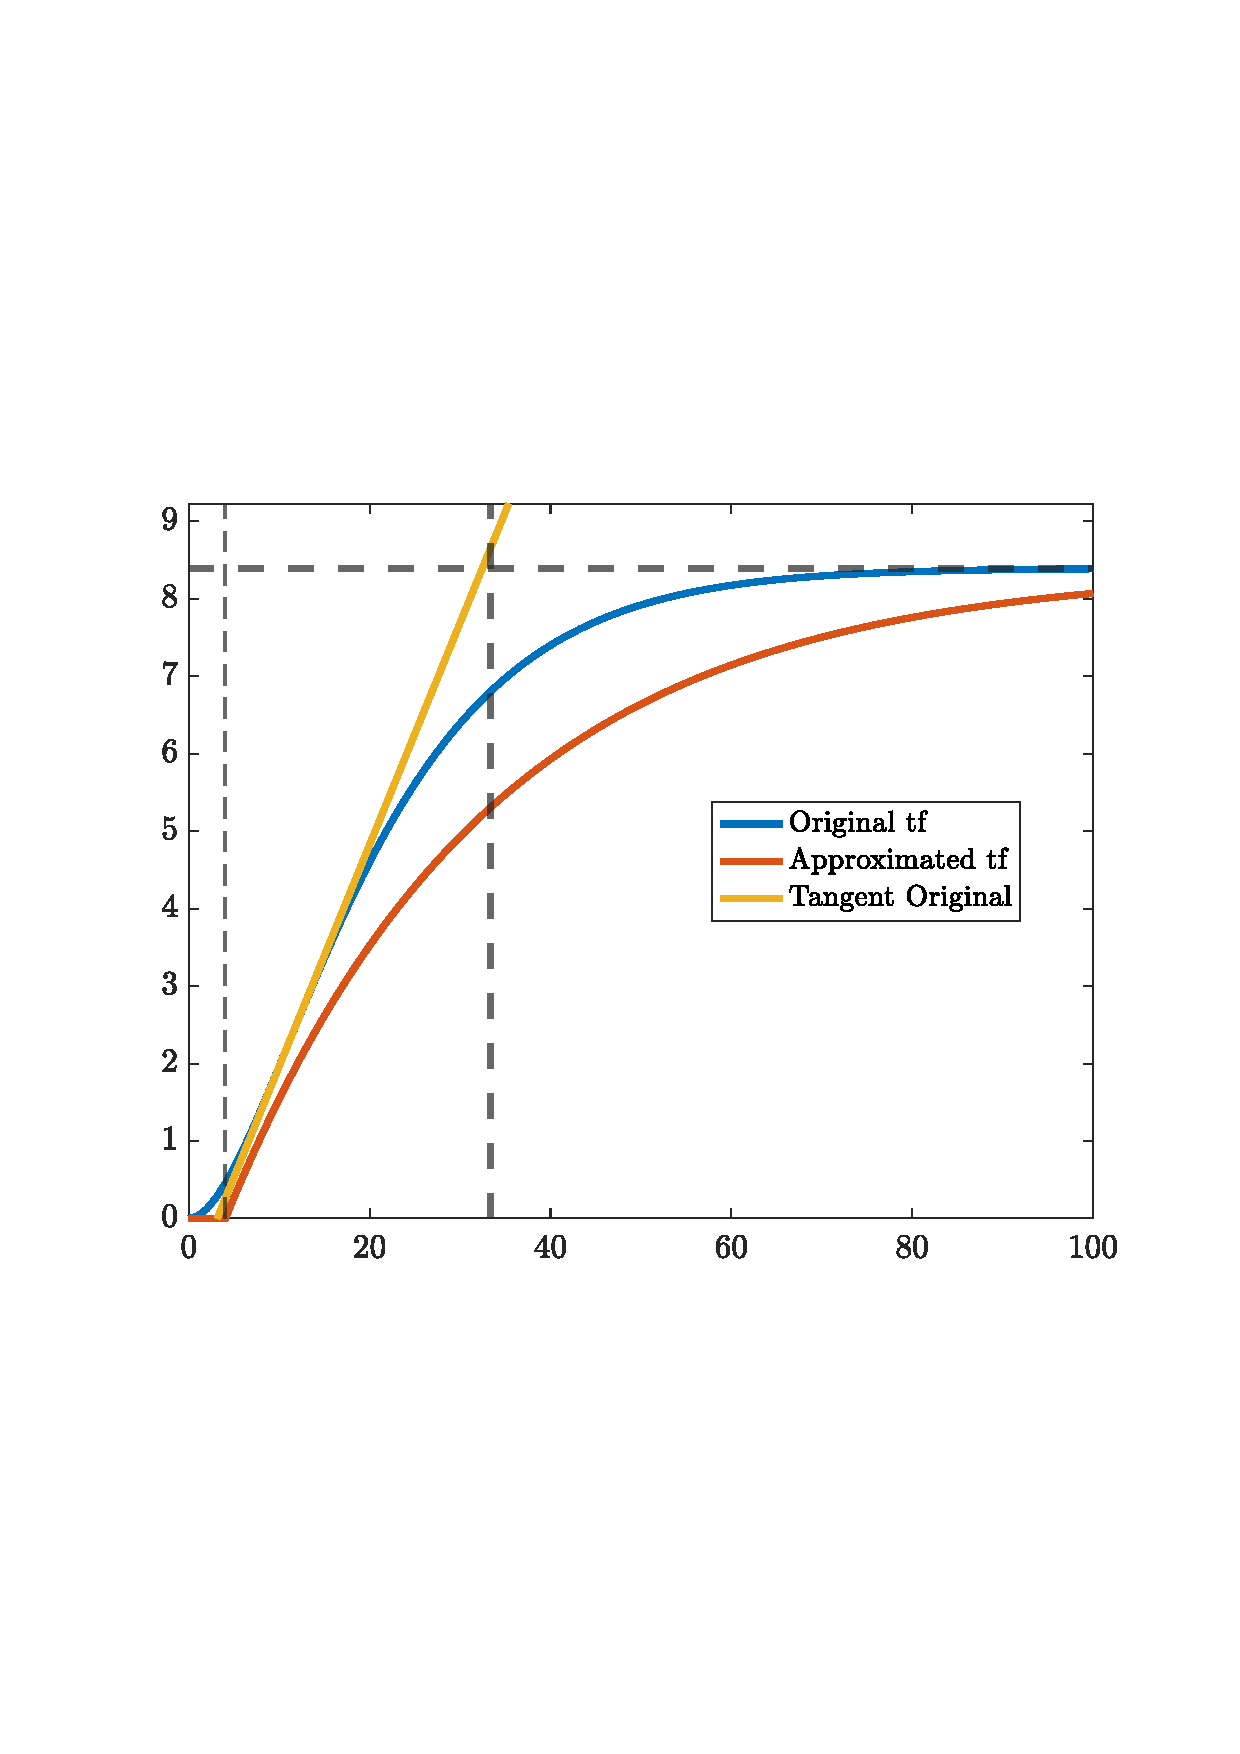
\includegraphics[width=1\linewidth, scale=1, trim=75 230 55 120,clip]{fig/G_11_max_slope_8ms.pdf}}
%
    \subcaptionbox{Two-point \label{fig:condes:ZN:results:2p_example}}[.48\textwidth]{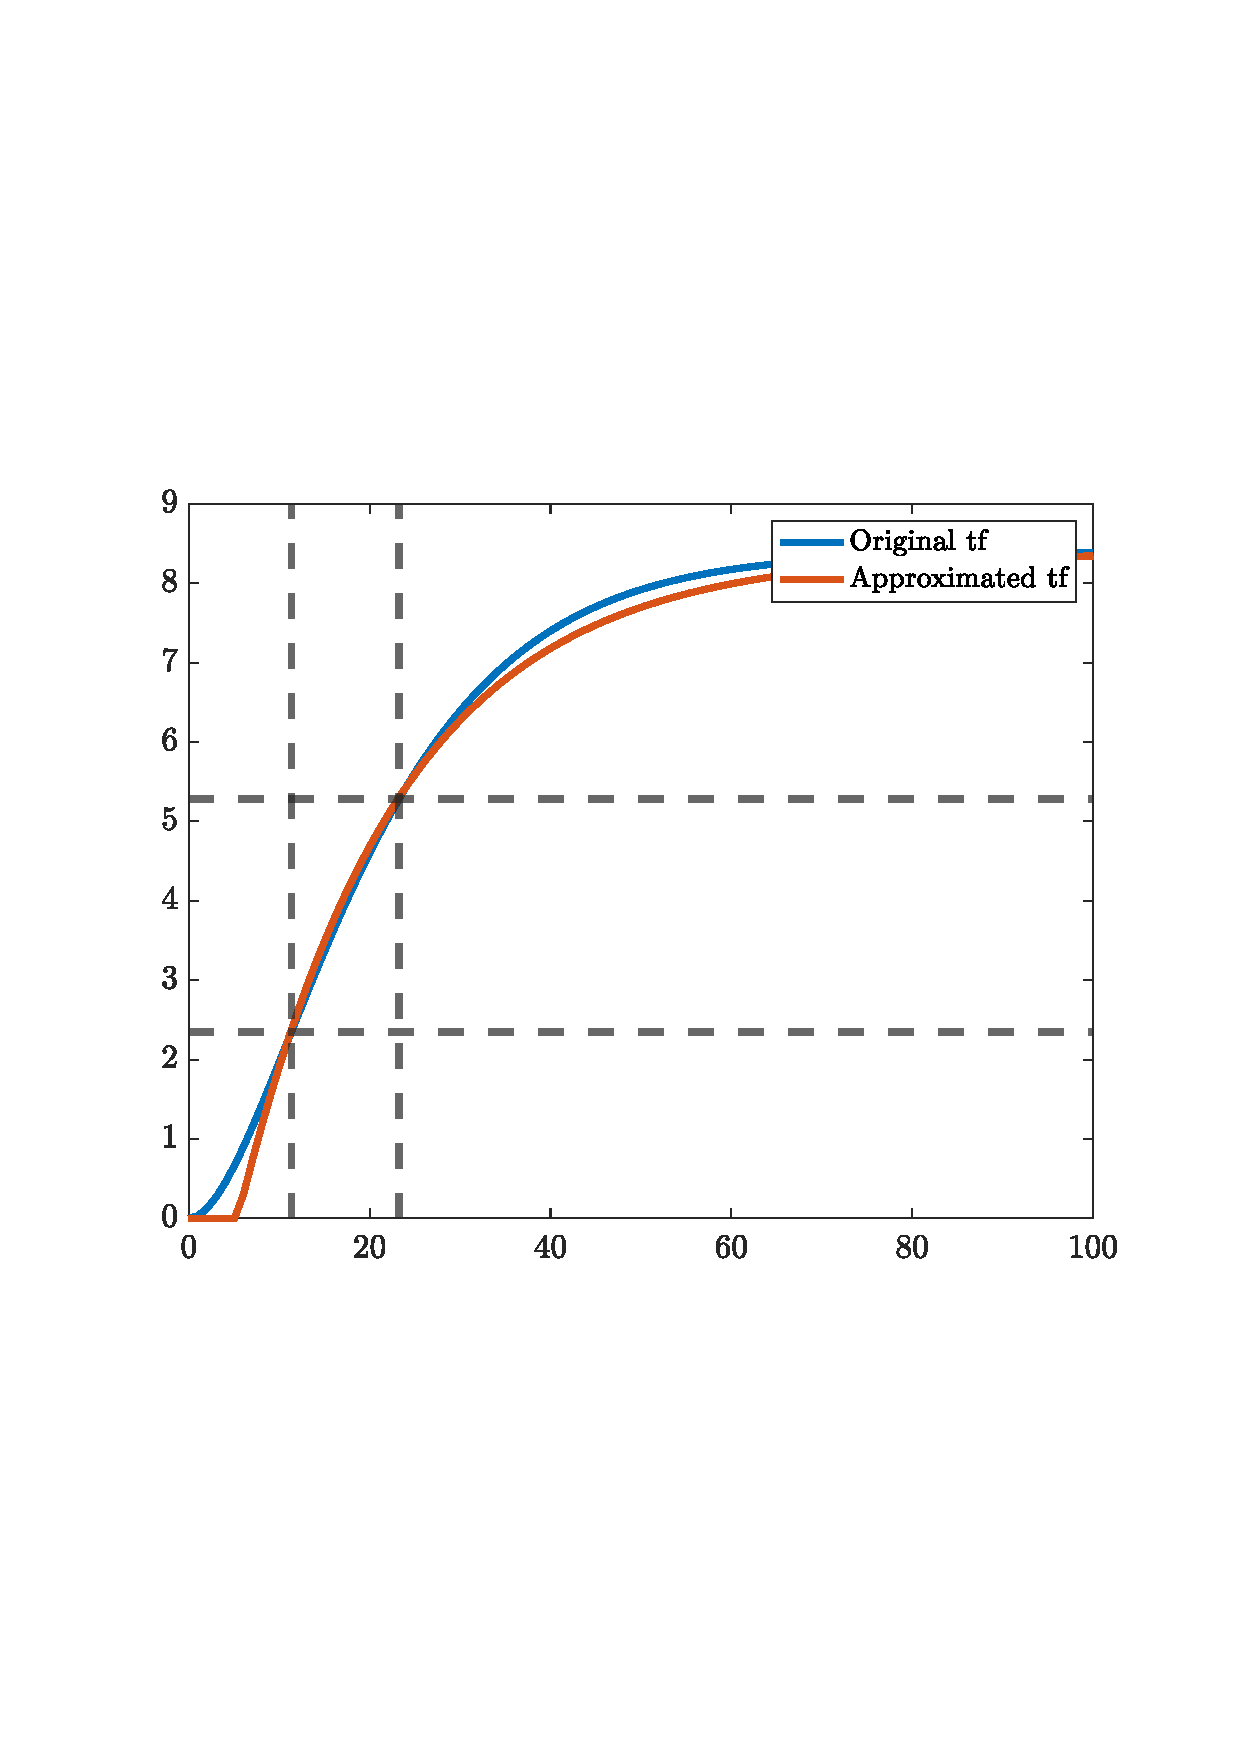
\includegraphics[width=1\linewidth, scale=1, trim=75 230 55 120,clip]{fig/G_11_2p_8ms.pdf}}

    \caption{Approximation of the transfer function at a wind speed of \SI{8}{\metre\per\second} and using the input-output pair 1-1}
    \label{fig:condes:ZN:results:example_plots}
\end{figure}

In \autoref{fig:condes:ZN:results:example_plots} we can clearly see the difference of approximation comparing max-slope and two-point method.
The result of the difference in approximation are different control parameter (\autoref{tab:condes:ZN:results}).
Still, the sign of all control parameters are equal and the differences are small.
When the wind speed is changed (using a different transfer function) the proportional factor $P$ of the PID controller changes.
The integral $I$ and derivative $D$ terms seem be constant.

\subsection{T-sum method} \label{sec:condes:Tsum}

For the input-output pair 2-2 we use the T-sum method.
T-Sum tries to find a line where two integrals have the same area. 
One is the area enclosed by the y-axis and the solution trajectory.
The other area is border by the solution trajectory and the $y_{\infty}$-value.
By shifting the dashed line seen in \autoref{fig:condes:tsum:example} on the $y$-axis the optimal point of equal areas is found.
The controller's parameters are calculated by $T_{\Sigma}$.
\begin{align}
    P &= \frac{1}{K} \\
    I &= 0.667 \cdot T_{\Sigma} \\
    D &= 0.167 \cdot T_{\Sigma}
\end{align}

\begin{table}[H]
    \caption{Results of PID controller design using T-Sum method.}
    \centering
    \begin{tabular}{ccccc} \toprule
        $v_{wind}$ [\si{\metre\per\second}] &$P$ & $I$ & $D$ & Input-Output pair \\ \midrule
        7 & 0.1724 & 0.6737 & 0.1687 & 2-2 \\
        8 & 0.1479 & 0.6737 & 0.1687 & 2-2 \\ 
        9 & 0.1240 & 0.6737 & 0.1687 & 2-2 \\ \bottomrule
    \end{tabular}
    \label{tab:condes:tsum:results}
\end{table}

\begin{figure}[H]
    \center
    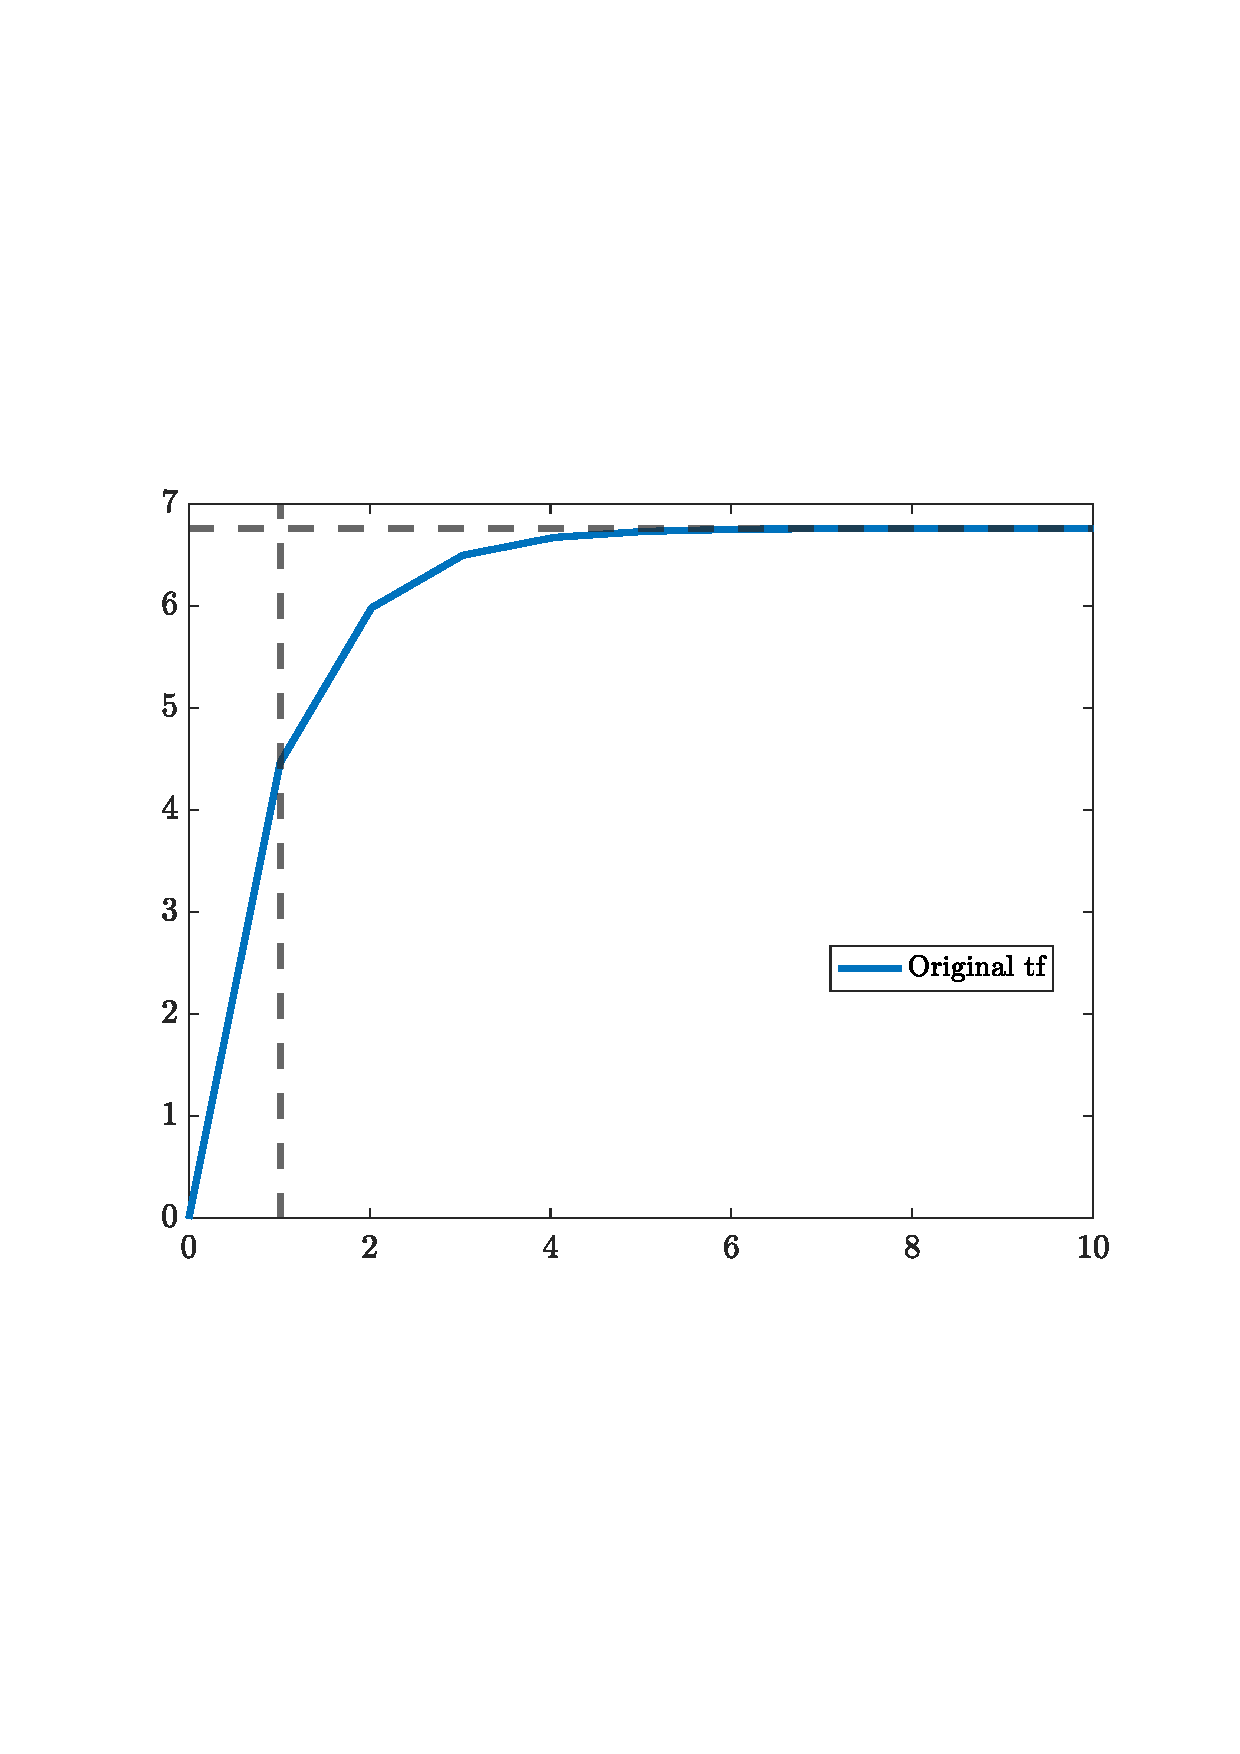
\includegraphics[scale=0.7,trim=60 200 50 150,clip]{fig/G_22_T_sum_8ms.pdf}
    \caption{Visualization of the T-sum method for controller design. A controller for the input-output pair 2-2 is designed by using the transfer function for a windspeed of \SI{8}{\metre\per\second}.}
    \label{fig:condes:tsum:example}
\end{figure}

%\autoref{fig:condes:tsum:example} shows one possible downside of the T-sum method. 
%When simulating the system the resulting solution is a discrete vector.

%\subsection{Relay-feedback method} \label{sec:condes:Relayfeedback}

\subsection{Implementation in Simulink} \label{sec:condes:implementation_simulink}

In the previous subsection the design of the controller is discussed.
Now, the implementation of the closed and open loop is addressed.
In contrast to the controller design, the closed and open loop is implemented in Simulink.

\subsubsection*{Open loop} \label{sec:condes:implementation_simulink:open_loop}

In general two different approaches for the implementation are possible.
The transfer function can be arranged as a structured flow diagram (\autoref{fig:condes:implementation:structure}).
In this case each transfer function is implemented individually in a single Simulink \texttt{tf-block}.
One advantage is that the overall structure of the system is visible and all \textit{flows of informations} are visible.
Otherwise, this implementation is more complex and therefore more error-prone.

The second case is a more condensed implementation (\autoref{fig:condes:implementation:block}).
In this, only two Simulink \texttt{LTI}-blocks are used for the system $G$ and the disturbance $G_D$.

\begin{figure}[H]
    \centering

    \subcaptionbox{Implementation as a structure \label{fig:condes:implementation:structure}}[.48\textwidth]{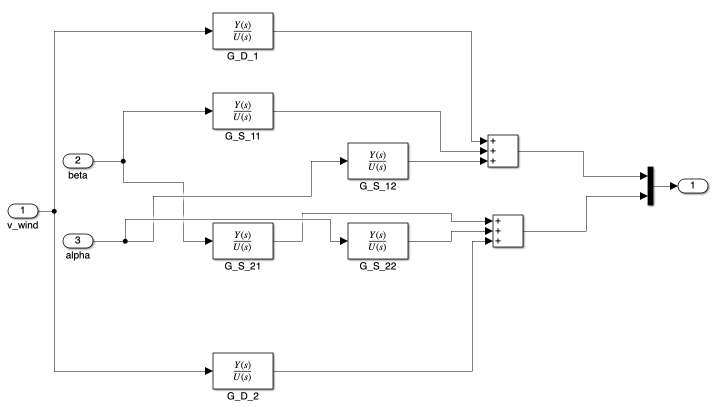
\includegraphics[width=1\linewidth, scale=1, trim=0 0 0 0,clip]{fig/Simulink/simulink_tf_structure.png}}
%
    \subcaptionbox{Implementation as blocks  \label{fig:condes:implementation:block}}[.48\textwidth]{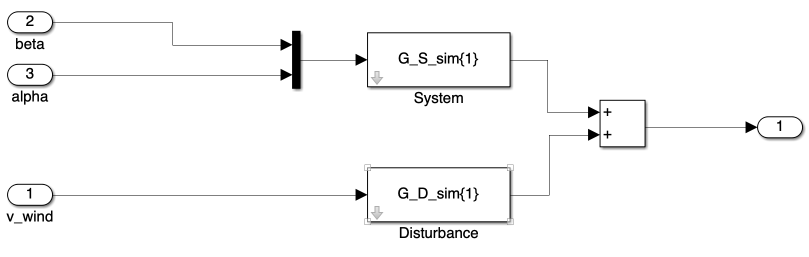
\includegraphics[width=1\linewidth, scale=1, trim=0 0 0 0,clip]{fig/Simulink/simulink_tf_block.png}}

    \caption{Comparing the two different approaches as Simulink block diagrams. The \textit{structured} implementation (\texttt{transfer\_function\_structured.slx}) reveals much more details about the internal dependencies. A more condensed view is seen for the \textit{block} implementation (\texttt{transfer\_function\_as\_block.slx}).}
    \label{fig:condes:implementation:two_approaches}
\end{figure}

To check the implementation it is good to use both implementation in parallel and check if both are getting the same results.
For further investigation the \textit{structured} implementation can be used.
This has the advantage that \textit{internal flows} or states can be monitored with Simulinks \texttt{scope}- or \texttt{out}-blocks.

\begin{figure}[H]
    \center
    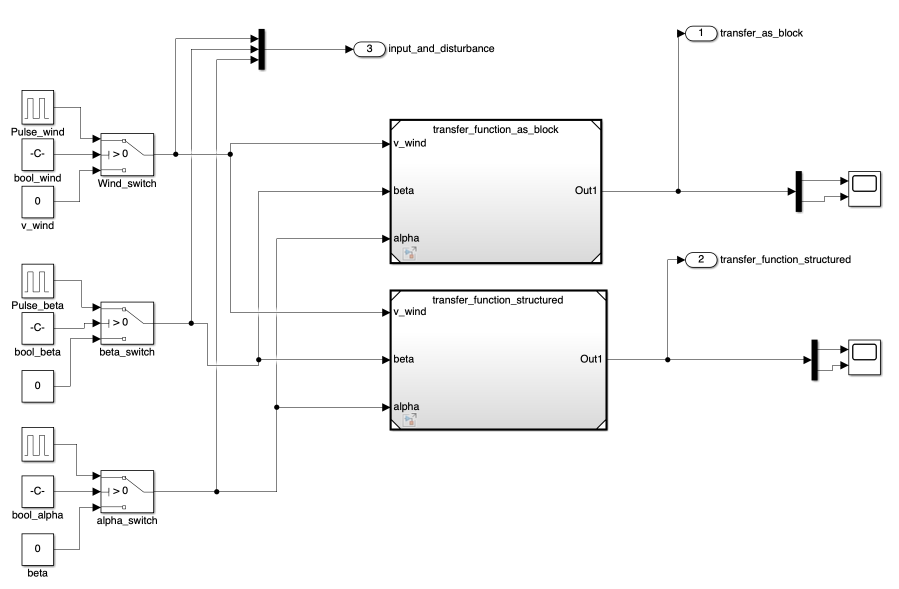
\includegraphics[width=1\textwidth,scale=1,trim=0 0 0 0,clip]{fig/Simulink/simulink_open_loop.png}
    \caption{The open loop system with a parallel execution of \textit{structured} and \textit{block} implementation. This figure is showing the \texttt{step\_response\_open\_loop.slx}-file.}
    \label{fig:condes:implementation:openloop}
\end{figure}

The Simulink file shown in \autoref{fig:condes:implementation:openloop} has three outputs.
\texttt{out1} returns the open loop behaviour for the \texttt{block} implementation, the second output (\texttt{out2}) for the \texttt{structured} implementation. 
The third \texttt{output}-block is to check the inputs into the system.

For each of the three inputs $v_{wind}$ (disturbance), $\beta$ and $\alpha$ (from top to down) a \texttt{switch}-block is used (see left side of the Simulink diagram).
These \texttt{switch}-blocks allow to choose via a flag set in a Matlab script which input should have a pulse applied to.
The pulse is produced by an \texttt{pulse}-block in Simulink.

\autoref{list:condes:implementation:flags} shows how to choose different scenarios depending on flags and \texttt{switch}-blocks.
Lines 7 ff. determine which pulse is given to system.
If the variable is set to $0$ the input does not have a pulse signal applied to, and it is constant $0$.
In the given example only $\beta$ will receive a pulse of magnitude \SI{7}{\degree} and a width of \SI{600}{\second} after \SI{600}{\second} of simulation time.

\begin{lstlisting}[style=Matlab-editor,caption={Setting flags for different combination of input pulses.},captionpos=b,label={list:condes:implementation:flags}]
% Setting amplitudes for pulse
simP.A_beta = 7;
simP.A_alpha = -.1;
simP.A_wind = -2;

% Determine if pulse of zero for inputs and disturbance
simP.bool_beta = 1;
simP.bool_alpha = 0;
simP.bool_wind = 0;

% Simulation paramters
simP.t_simulation = 2000; % Time for simulation [s]
simP.T_period = 1200;     % Peroid of pulse [s]
simP.T_delay = 600;       % Delay for first pulse [s]
simP.pulse_width = 50;    % Pulse width in % of T_Period [%]
\end{lstlisting}


\subsubsection*{Closed loop} \label{sec:condes:implementation_simulink:closed_loop}

When the designed controllers are tested the loop must be closed.

\begin{figure}[H]
    \center
    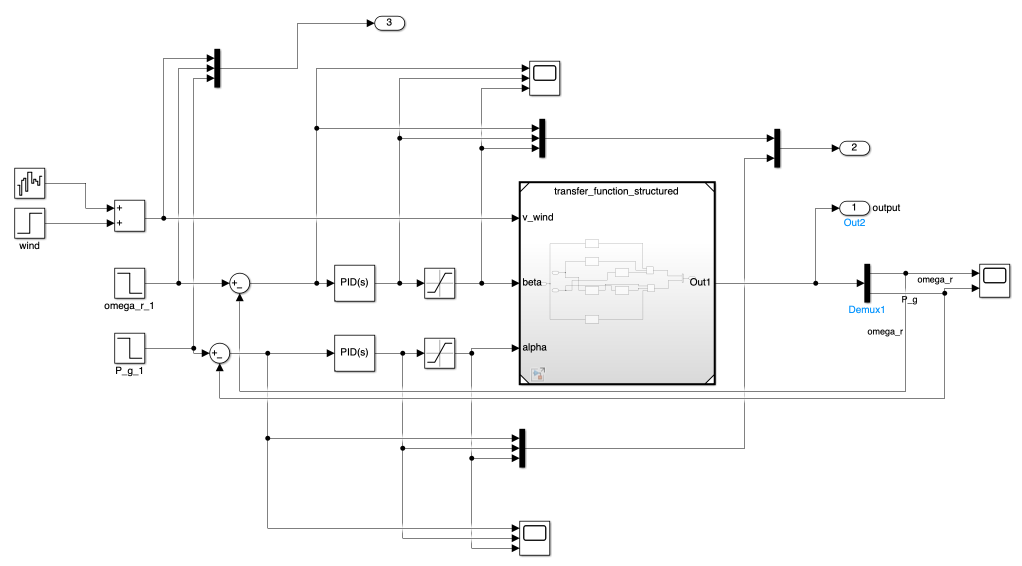
\includegraphics[width=1\textwidth,scale=1,trim=0 0 0 0,clip]{fig/Simulink/simulink_closed_loop.png}
    \caption{The closed loop with a \texttt{PID}-controller block, both reference signals and a possible disturbance due to wind. This figure is showing the \texttt{closed\_loop\_PID.slx}-file.}
    \label{fig:condes:implementation:closedloop}
\end{figure}

For possible disturbance due to a change in wind speed a \texttt{step}- and a \texttt{noise}-block is added.
With this setup, not only can the wind change drastically (step change, boe) but also naturally occurring fluctuation can be simulated.
After the \texttt{PID}-block a \texttt{saturation}-block is added.
\autoref{sec:condes:discussion} discusses the need of having a saturation block, which enforces the limitations of input signals shown in \autoref{tab:analysis:constraints}.


%\include{src/1_system_derivation}
%\include{src/2_controler_design}
%\include{src/3_model_discretization}
%\include{src/4_simulation_results}

\bibliographystyle{plain}
\bibliography{bibliography/my_bib.bib}


\end{document}